\documentclass[12pt,a4paper]{article}

\usepackage[english,russian]{babel}
\usepackage[utf8]{inputenc}
\usepackage{amsmath}
\usepackage{graphicx}
\usepackage[colorinlistoftodos]{todonotes}
\usepackage{indentfirst}
\usepackage{tikz}
\usepackage[T1]{fontenc}
\usepackage{mathptmx}
\usepackage{geometry}
\usepackage{subfigure}

\usetikzlibrary{shapes,arrows}

\linespread{1.5}

\geometry{left=3cm}
\geometry{right=2cm}
\geometry{top=2cm}
\geometry{bottom=2cm}

\bibliographystyle{unsrt}


\renewcommand{\Re}{\mathop{\mathrm{Re}}\nolimits}
\renewcommand{\Im}{\mathop{\mathrm{Im}}\nolimits}


\title{Стабилизация плавательного средства}

\author{Влад Агиевич}

\date{\today}

\begin{document}

\begin{titlepage}

\begin{center}
Министерство образования и науки Российской Федерации \\
Федеральное государственное автономное образовательное учереждение высшего профессионального образования \\
<<Московский физико-технический институт(государственный университет)>> \\
Факультет аэрофизики и космических исследований \\
Кафедра технической кибернетики \\
\end{center}

\vspace{8mm}

\vspace{8mm}

\begin{center}
Агиевич Владислав Николаевич \\
{\large Стабилизация плавательного средства \\[8mm]
{\bf Магистерская диссертация\\}
}
\end{center}

\vspace{8mm}

\vspace{10mm}

\begin{center}
г. Москва
\end{center}
\begin{center}
2016
\end{center}
\end{titlepage}

\newpage

\tableofcontents

\newpage

\section{Введение} 


\begin{figure}[ht!]  
	\vspace{4ex} 
	\centering \subfigure[]{
		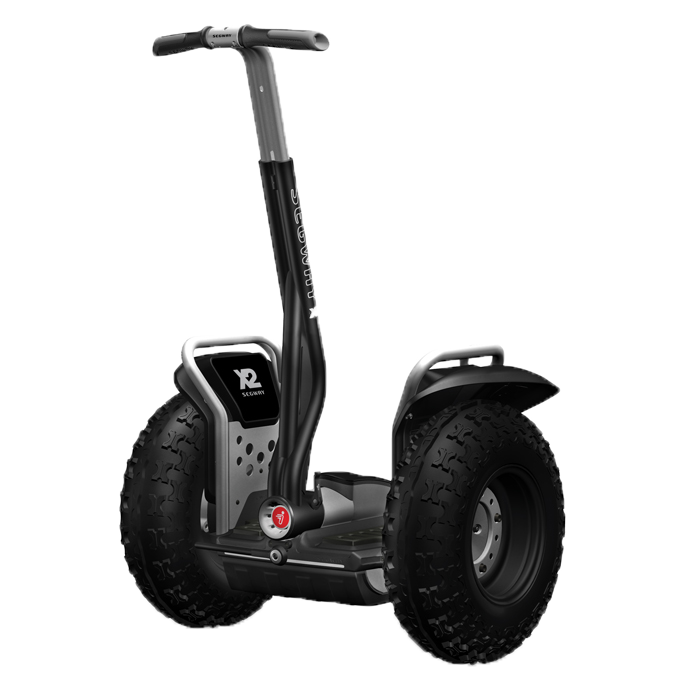
\includegraphics[width=0.25\linewidth]{images/segway.png} \label{fig:segway} 
	}  
	\hspace{4ex}
	\subfigure[]{
		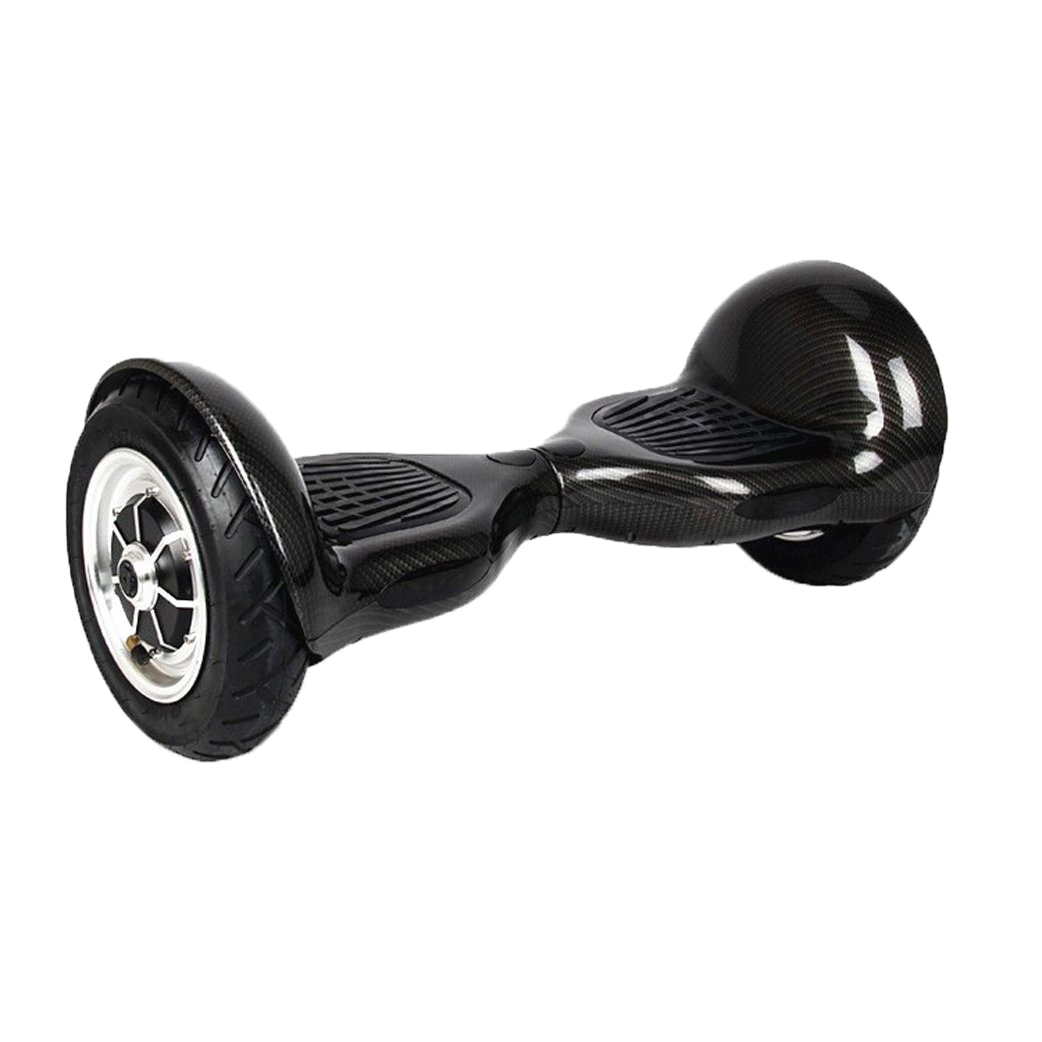
\includegraphics[width=0.25\linewidth]{images/gyroboard.png} \label{fig:gyroboard} 
	}
	\hspace{4ex}
	\subfigure[]{ 
		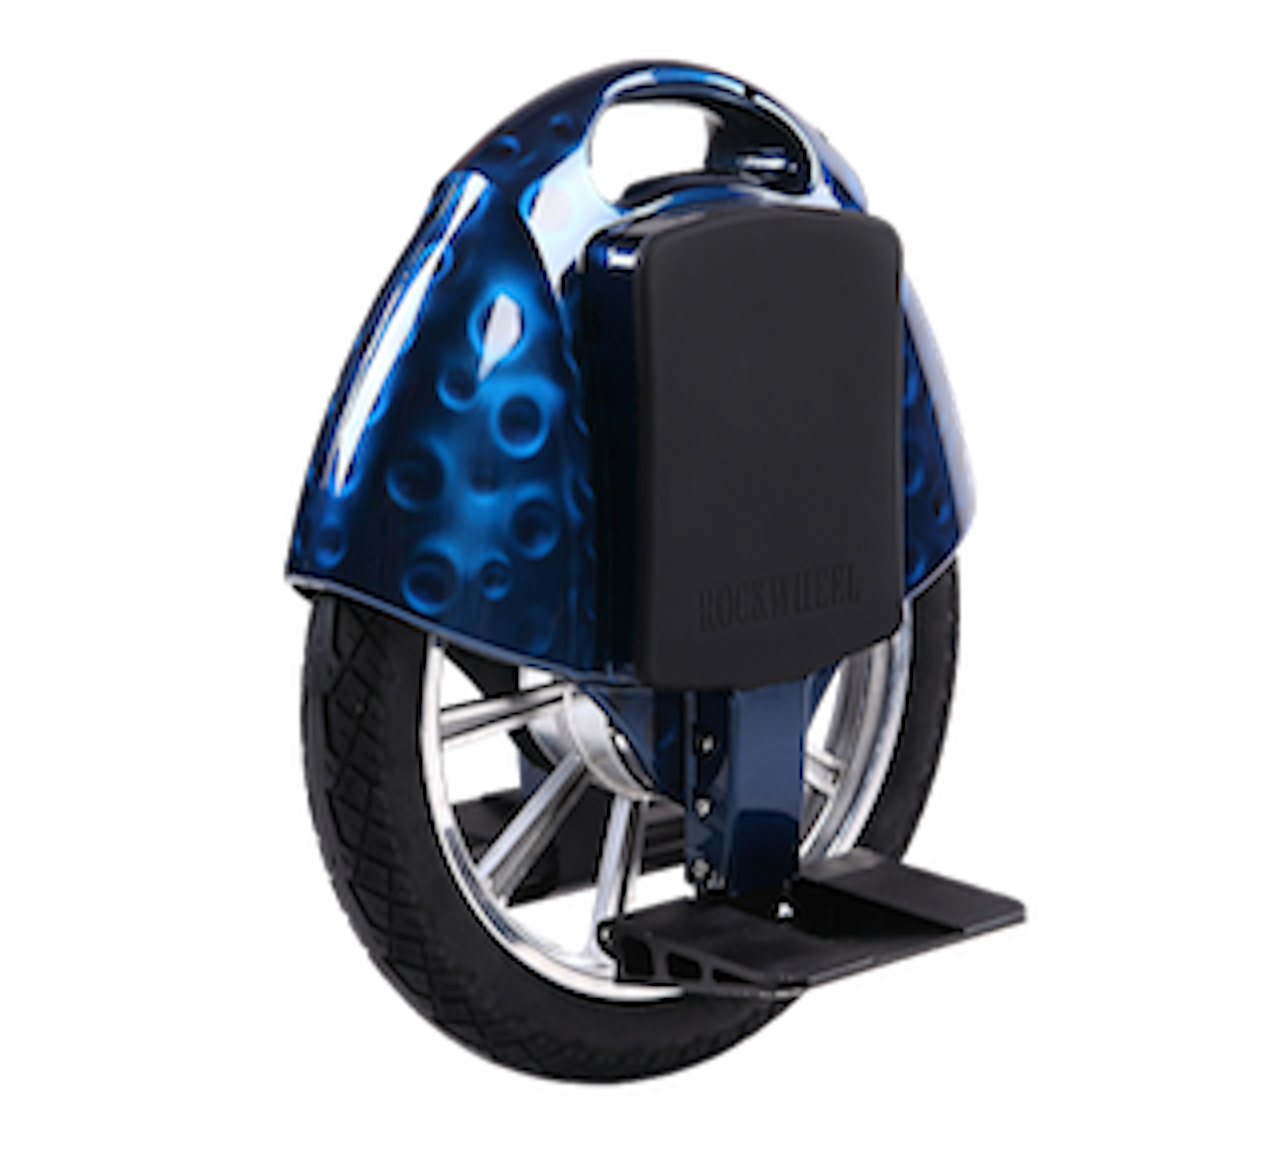
\includegraphics[width=0.24\linewidth]{images/rockwheel.png} \label{fig:rockwheel} 
	}  
	\caption{Новые средства передвижения: \subref{fig:segway} сегвэй; \subref{fig:gyroboard} гироборд; \subref{fig:rockwheel} моноколеса} 
	\label{fig:new_transport}
\end{figure}


В настоящее время большой интерес вызывают средства передвижения, основанные на балансировании (см.~рис.~$\ref{fig:new_transport}$). На земле это сегвеи - два колеса и ручка, гироборды - просто два колеса, и даже моноколеса. Весь этот транспорт реагирует на наклон человека как на управляющее воздействие и, благодаря вращению колес, движется вперед, не давая человеку упасть. Плавательных средств, основанных на таком принципе еще нет. Во всяком случае, средств получивших широкое распространение. Возможно, потому что при движении по воде у транспортного средства есть две степени свободы: бортовая качка и килевая качка (см.~рис.~$\ref{fig:kachka}$). С качкой борется целый раздел теории корабля под названием остойчивость. 

\begin{figure}[h]
	\centering 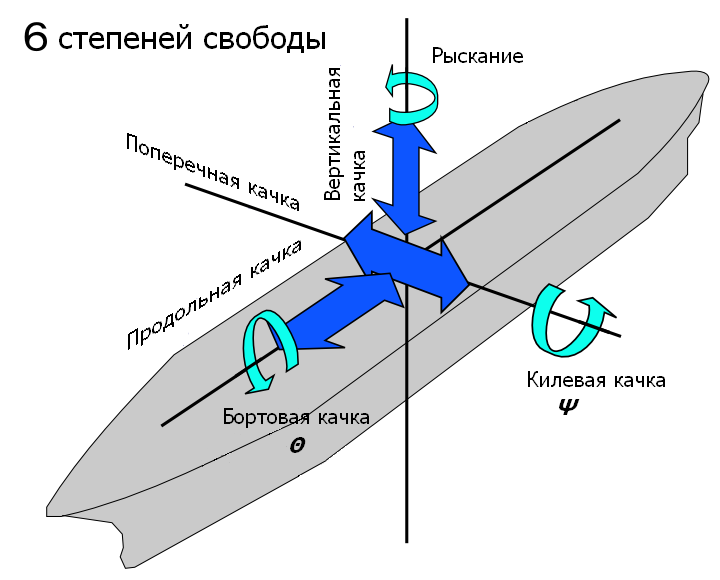
\includegraphics[width=0.4\linewidth]{images/kachka.png}
	\caption{Виды качки}
	\label{fig:kachka}
\end{figure}
Применяя закон изменения момента импульса легко получить следующее утверждение. Если центр масс плавательного средства находится глубже, чем центр плавучести (центр масс погруженной в воду части), то плавательное средство остойчиво. Если же нет, то тогда нужна некоторая дополнительная стабилизация.

Для построения плавательного средства с системой активной стабилизации необходимо математическое описание.

Описание средств передвижения - не новая тема. Существуют математические модели кораблей, вертолетов и т.п. Модели значительно облегчают управление и навигацию транспортных средств Но что если транспортное средство достаточно примитивно, например, доска для серфинга, а существующие модели лодок и кораблей слишком громоздки? Нужно строить свою.


\section{Постановка задачи}

Из вышесказанного следует, что конструирование плавательного доски, позволяющей человеку передвигаться стоя, является весьма перспективной задачей. Одним из первых этапов разработки являются моделирование и прототипирование. Данная работа посвящена прототипированию плавательной доски с системой активной стабилизации, а также обзору некоторых задач, встающих перед перед разработчиками роботизированных систем и автоматического транспорта

Работа поделена на следующие этапы:

\begin{itemize}
	\item Построение структурной модели
	\item Параметрическая идентификация
	\item Стабилизация
\end{itemize}

Прототипирование должно ответить на вопрос: возможно ли, в принципе, сконструировать плавательное средство с высоким центром тяжести, устойчивое относительно продольной качки, и опробовать технологии и алгоритмы для создания полноразмерной доски.

Чтобы построение прототипа было осмысленным, а результат был неслучайным, в первую очередь необходимо понять с чем мы работаем и в чем состоит задача с математической точки зрения.

\begin{figure}
	\tikzstyle{block} = [draw, rectangle, 
	    minimum height=3em, minimum width=6em]
	\tikzstyle{sum} = [draw, circle, node distance=1cm]
	\tikzstyle{input} = [coordinate]
	\tikzstyle{output} = [coordinate]
	\tikzstyle{pinstyle} = [pin edge={to-,thin,black}]

	\centering
	% The block diagram code is probably more verbose than necessary
	\begin{tikzpicture}[auto, node distance=2cm,>=latex']
	    % We start by placing the blocks
	    \node [input, name=input] {};
	    \node [sum, right of=input] (sum) {};
	    \node [block, right of=sum] (controller) {Регулятор};
	    \node [block, right of=controller, pin={[pinstyle]above:Возмущения},
	            node distance=3cm] (system) {Объект};
	    % We draw an edge between the controller and system block to 
	    % calculate the coordinate u. We need it to place the measurement block. 
	    \draw [->] (controller) -- node[name=u] {$u$} (system);
	    \node [output, right of=system] (output) {};
	    \node [block, below of=u] (measurements) {Измерения};

	    % Once the nodes are placed, connecting them is easy. 
	    \draw [draw,->] (input) -- node {$r$} (sum);
	    \draw [->] (sum) -- node {$e$} (controller);
	    \draw [->] (system) -- node [name=y] {$y$}(output);
	    \draw [->] (y) |- (measurements);
	    \draw [->] (measurements) -| node[pos=0.99] {$-$} 
	        node [near end] {$y_m$} (sum);
	\end{tikzpicture}
	\caption{Типичная схема в задачах автоматического управления}
	\label{fig:typical_auto_control}
\end{figure}

С такими схемами как на рис.~$\ref{fig:typical_auto_control}$ обычно работают в теории автоматического управления. Известно описание объекта, либо в виде передаточных функций, либо в пространстве состояний и задача стабилизации состоит в том, чтобы подобрать регулятор, который сделает замкнутую систему устойчивой. Случай регуляторов простой формы и общий случай рассмотрены в \cite{polyak_scherbakov_robust}.

В реальности же мы имеем схему на рис.~$\ref{fig:my_process}$.

\begin{figure}
	\tikzstyle{block} = [draw, rectangle, 
	    minimum height=3em, minimum width=6em]
	\tikzstyle{sum} = [draw, circle, node distance=1cm]
	\tikzstyle{input} = [coordinate]
	\tikzstyle{output} = [coordinate]
	\tikzstyle{pinstyle} = [pin edge={to-,thin,black}]
	
	\centering
	\begin{tikzpicture}[auto, node distance=2cm,>=latex']
	    \node [input, name=input] {};
	    \node [sum, below of=input] (sum1) {};
	    \node [block, below of=sum1] (controller) {Регулятор};

	    \node [block, below left = 10mm and -8mm of controller] (motor_controller_left) {Контроллер мотора};
	    \node [block, below right = 10mm and -8mm of controller] (motor_controller_right) {Контроллер мотора};

	    \node [block, below = 10mm of motor_controller_left] (motor_left) {Мотор};
	    \node [block, below = 10mm of motor_controller_right] (motor_right) {Мотор};

	    \node [sum, below = 6 cm of controller] (sum2) {};

	    \node [block, below = 10mm of sum2, pin={[pinstyle]right:Возмущения},
	            node distance=3cm] (system) {Доска};

	    \draw [draw,->] (input) -- node {Угол уставки} (sum1);
	    \draw [->] (sum1) -- node {$e$} (controller);

	    \draw [->] (sum2) -- node {Тяга} (system);

	    \draw [->] (motor_right.south) |-  
	        node [above, near end] {$F_r$} (sum2.east);
	    \draw [->] (motor_left.south) |- node[pos=0.96] {$-$} 
	        node [above, near end] {$F_l$} (sum2.west);

	    % стрелки от регулятора к контроллерам моторов
	    \draw [->] (controller.west) -| node [left, near end] {Внутр. сигнал}  (motor_controller_left.north);
	    \draw [->] (controller.east) -| node [right, near end] {Внутр. сигнал}  (motor_controller_right.north);

	    % стрелки от контроллеров моторов к моторам
	    \draw [->] (motor_controller_left) -- node [left] {Внутр. сигнал} (motor_left);
	    \draw [->] (motor_controller_right) -- node [right] {Внутр. сигнал} (motor_right);

	    % выходной сигнал
	    \node [output, below = 15 mm of system] (output) {};

	    % измерительный блок
	    \node [block, left = 35 mm of motor_left, rotate=90, anchor=north] (measurements) {Измерительный блок};

	    \draw [->] (measurements) |- node[pos=0.98] {$-$} 
	        node [near end] {$y_m$} (sum1);

	    \draw [->] (system) -- node [name=y] {Угол}(output);
	    \draw [->] (y) -| (measurements);

	\end{tikzpicture}
	\caption{Схема процесса}
	\label{fig:my_process}
\end{figure}

Таким образом, наша задача состоит в том, чтобы соотнести две схемы: т.е. преобразовать блоки рис.~$\ref{fig:my_process}$ в блоки рис.~$\ref{fig:typical_auto_control}$.
Начнем с измерительного блока.

\section{Конструкция}

Вообще, есть два варианта конструкции: с штангой и с килем. Схематически их можно представить в виде рис.~$\ref{fig:shtanga}$~и~$\ref{fig:kil}$. Они отличаются лишь местом, в котором мы генерируем компенсирующий момент. Для плавания более удобен вариант с килем, но, в то же время, правильный киль сложнее изготовить, поэтому при прототипировании мы ограничились моделью со штангой.

\begin{figure}[h!]
	\center{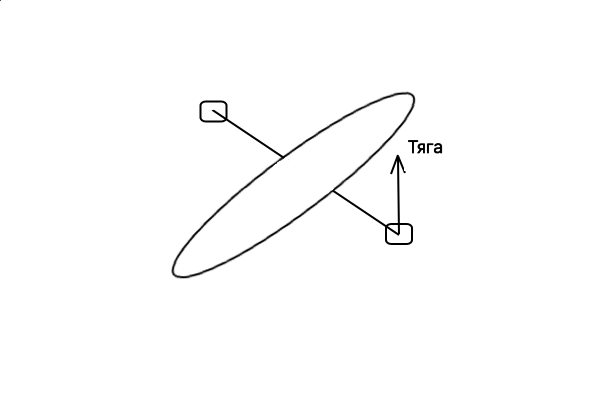
\includegraphics[width=1\linewidth]{images/shtanga.png}}
	\caption{Доска со штангой}
	\label{fig:shtanga}
\end{figure}

\begin{figure}[h!]
	\center{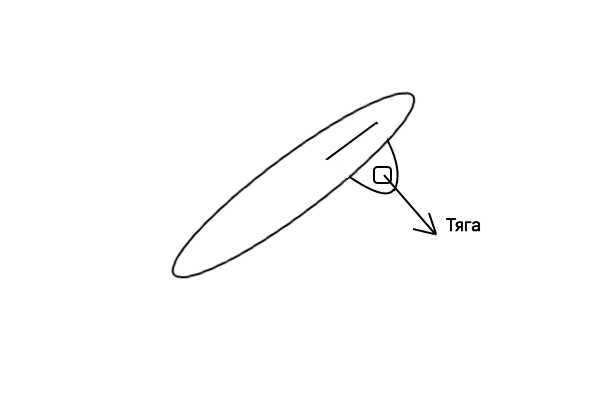
\includegraphics[width=1\linewidth]{images/kil.png}}
	\caption{Доска с килем}
	\label{fig:kil}
\end{figure}

\begin{figure}[h!]
	\center{\includegraphics[width=0.6\linewidth]{images/boat_photo_scheme.png}}
	\caption{Устройство прототипа плавательного средства}
	\label{fig:boat_photo_scheme}
\end{figure}

Из рис. $\ref{fig:boat_photo_scheme}$ видно, что основными элементами конструкции являются:
\begin{itemize}
	\item Корпус из пенопропилена
	\item Мачта (для крепления грузов)
	\item Батарея
	\item Управляющая электроника
	\item Контроллеры моторов
	\item Моторы и винты на них
\end{itemize}

Коробка с управляющей электроникой набита поролоном для того, чтобы гасить вибрации, исходящие от моторов.



\section{Описание алгоритма}

На мачту из рис. $\ref{fig:boat_photo_scheme}$ крепится какой-нибудь неравномерный груз для того, чтобы создать переворачивающий момент. Измеряя угол и угловую скорость мы генерируем тягу на винтах, чтобы скомпенсировать переворачивающий момент.

\begin{figure}[h!]
	\center{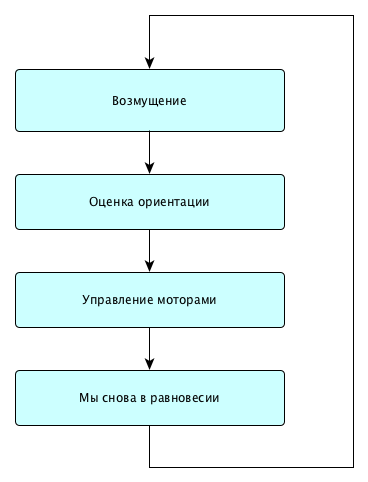
\includegraphics[width=0.7\linewidth]{images/general_scheme.png}}
	\caption{Общая схема процесса}
	\label{fig:general_scheme}
\end{figure}

Фактически схема~$\ref{fig:general_scheme}$ выглядит следующим образом (см.~рис.~$\ref{fig:advanced_scheme}$ )

\begin{figure}[h!]
	\center{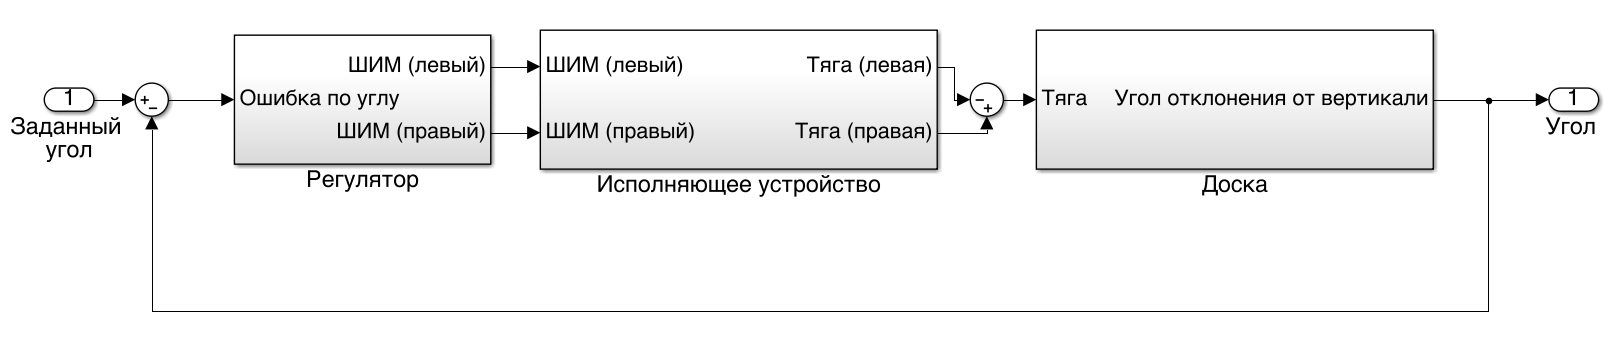
\includegraphics[width=1\linewidth]{images/advanced_scheme.png}}
	\caption{Более подробная схема процесса}
	\label{fig:advanced_scheme}
\end{figure}

А исполняющее устройство:

\begin{figure}[h!]
	\center{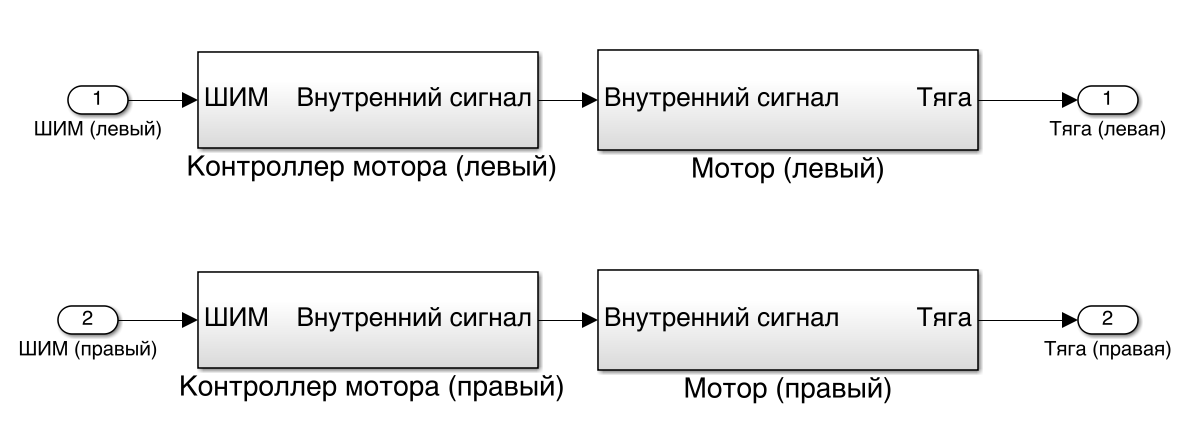
\includegraphics[width=1\linewidth]{images/isp_ustr.png}}
	\caption{Исполняющее устройство}
	\label{fig:isp_ustr}
\end{figure}

\section{Набор датчиков}

Для оценки ориентации твердого тела в пространстве часто используется набор из трех датчиков: акселерометра, гироскопа и магнитометра. Акселерометр измеряет ускорение тела, как динамическое - собственно движение, так и статическое - гравитацию. Гироскоп, точнее датчик угловой скорости, измеряет угловую скорость. А магнитометр измеряет направление и величину магнитного поля.

В наших экспериментах, в качестве управляющего устройства и обработчика измерений мы использовали уже готовую платформу Pixhawk 2.4.8. Она снабжена следующими датчиками:

MPU-6000. Акселерометр и ДУС в одном корпусе. Трехосевой акселерометр может измерять ускорение с 16-битным разрешением в диапазонах $\pm$2g, $\pm$4g, $\pm$8g, $\pm$16g. Трехосевой датчик угловой скорости также может проводить измерения с 16-битным разрешением в различных диапазонах: $\pm250$, $\pm$500, $\pm$1000, $\pm$2000 $^\circ /sec$. Оба датчика имеют настраиваемый встроенный фильтр нижних частот.

L3GD20. ДУС с разрешением 16 бит и выбором диапазона $\pm250$, $\pm$500, $\pm$2000 $^\circ /sec$. Также имеет встроенные настраиваемые фильтры нижних и верхних частот.

HMC5883L. Магнитометр с разрешением 12 бит.

\subsection{Калибровка}

Датчики с архитектурой MEMS (Micro Electro Mechanical System) достаточно дешевы, поэтому зачастую требуют калибровки перед использованием. Калибровка подразумевает, что существует истинное значение измеряемой величины, а измеряем мы некоторое искаженное значение. Соответсвенно, ее задача состоит в том, чтобы нивелировать искажение. В наших экспериментах калибровка проводилась при помощи программы с открытым исходным кодом QGroundControl, но я считаю важным рассказать о том как же решается эта задача, потому что решал ее и самостоятельно в течение работы.

\subsubsection{Акселерометр}

Начнем с акселерометра. В неподвижном положении он измеряет исключительно гравитацию. Поэтому зная положение датчика в пространстве, мы знаем и его истинные показания.

Например, на рис. (вставить рисунок) истинные показания акселерометра должны быть $(0, 0, g)$. Измеряемое значение ускорения может отличаться по ряду причин:

\begin{itemize}
	\item Смещение показаний
	\item Различная чувствительность осей
	\item Неортогональность осей датчика
	\item Несовпадение по направлению осей глобальной СК и осей датчика
\end{itemize}

Под глобальной СК имеется в виду СК платы, на которой находится сенсор или СК коробки, в которой он лежит.

Можно учесть все эти параметры по отдельности, выделив три отдельных матрицы:

$$ \vec{a}_{\text{изм}} = M_{\text{поворота между двумя СК}} M_{\text{ортогонализации}} K \vec{a}_{\text{ист}} + \vec{b},$$

где $K$ - диагональная матрица чувствительностей, а $\vec{b}$ - смещение показаний.

А можно и объединить три матрицы в одну:

$$ \vec{a}_{\text{изм}} = F_{\text{искажения}}\vec{a}_{\text{ист}} + \vec{b} $$

Зная $\vec{a}_{\text{ист}}$ в нескольких точках, например, совмещая различные оси датчика с направлением гравитации, можно составить систему линейных уравнений относительно параметров искажения, которых у нас 12 (9 элементов матрицы искажения и 3 элемента вектора постоянного сдвига). Если точек больше четырех, то получится переопределенная система, которую легко решить методом наименьших квадратов.

В результате, зная матрицу $F_{\text{искажения}}$ и вектор $\vec{b}$, мы можем из зашумленных измеренных данных получить настоящие ускорения.

$$ \vec{a}_{\text{ист}} = F_{\text{искажения}}^{-1}(\vec{a}_{\text{изм}} - \vec{b})  $$

\subsubsection{Магнитометр}

Искажения магнитометра математически выглядят также как и у акселерометра, но их источником является не только неидельность производства, а и массивные железные объекты и токи вблизи сенсора, вносящие неоднородность в магнитное поле.

Основная сложность состоит в том, что мы изначально не знаем куда направлено магнитное поле Земли. Но мы можем воспользоваться общим для для трехосевых датчиков, измеряющих векторные поля, правилом: модуль измеряемого вектора сохраняется при различных поворотах в пространстве.

$$ |\vec{m}|^2 = m_x^2 + m_y^2 + m_z^2 = const $$

Таким образом при всех возможных вращениях датчика, вектор магнитной индукции должен описать сферу с центром в начале координат в системе отсчета, связанной с датчиком. Но это случится только при идеальном сенсоре. В реальности же сфера превратится в эллипсоид и центр сдвинется из начала координат.

\begin{figure}[h!]
	\center{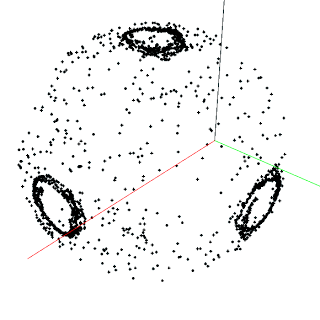
\includegraphics[width=0.7\linewidth]{images/compass_points.png}}
	\caption{Набор измерений магнитометра}
	\label{fig:compass_points}
\end{figure}

Отсюда вытекает метод калибровки магнитометра, который учитывает все искажения акселерометра кроме несовпадения осей. 

\begin{enumerate}
	\item Собрать равномерный набор точек
	\item Аппроксимировать их эллипсоидом
	\item Вычислить обратное преобразование из полученного эллипсоида в единичную сферу с центром в начале координат
	\item Применить обратное преобразование, вид которого будет таким же, как и для акселерометра
\end{enumerate}

$$ \vec{m}_{\text{ист}} = F_{\text{искажения}}^{-1}(\vec{m}_{\text{изм}} - \vec{b}) $$

В задаче оценки ориентации нам не важно абсолютное значение магнитного поля, поскольку повороты в пространстве не изменяют длины векторов.

Чтобы вычислить матрицу поворота между глобальной системой координат и системой координат датчика, необходимо совершить вращение вокруг оси глобальной СК при двух противоположных положениях датчика. Если совместим центры двух полученных кругов, то получим вектор, в которых переходит орт глобальной системы координат.

\section{Оценка ориентации}

\subsection{Фильтр Калмана}

Фильтр Калмана для линейной дискретной системы:
\begin{align}
	\label{eq:kalman_state_evolution} \boldsymbol x_{k+1} &= \boldsymbol A_k \boldsymbol x_k + \boldsymbol w_k \\ 
	\label{eq:kalman_measurement} \boldsymbol z_k &= \boldsymbol H_k \boldsymbol x_k + \boldsymbol v_k, \\
\notag
\end{align}

где $x_k \in R^n$ - состояние, а $z_k \in R^m$ - измерение. Шум процесса $w_k$ и шум измерений $v_k$ считаем независимыми случайными величинами с гауссовской функцией плотности вероятности и нулевым средним. Нормальные распределения вероятности $p$ в таком случае

\begin{align*}
	\boldsymbol p(\boldsymbol w) \sim N(0,\boldsymbol Q) &, \boldsymbol Q = diag\{ \sigma^2_{w_1}, \sigma^2_{w_2}, \dots \} \\
	\boldsymbol p(\boldsymbol v) \sim N(0,\boldsymbol R) &, \boldsymbol R = diag\{ \sigma^2_{v_1}, \sigma^2_{v_2}, \dots \}
\end{align*}

$\sigma^2$ - дисперсии соответствующих распределений. $\boldsymbol A_k$ - матрица $n \times n$, описывающая переход системы между временами $k$ и $k+1$ при отсутствии входного сигнала и шума процесса. $\boldsymbol H_k$ - матрица $m \times n$, соотносящая состояние $\boldsymbol x_k$ с измерением $\boldsymbol z_k$. Фильтр состоит из двух стадий. Первая стадия состоит в предсказании состояния $\hat{x}_k^-$ на шаге $k$, используя матрицу динамики системы $\boldsymbol A_{k-1}$ и состояние $\boldsymbol x_{k-1}$ с предыдущего, $k-1$-го, шага. В дальнейшем мы будем называть $\hat{\boldsymbol x}_k^-$ оценкой a priori. Вторая - корректировка этой оценки с использованием измерения $\boldsymbol z_k$. Можно ввести новую переменную (невязку)

$$ \boldsymbol y_k = \boldsymbol z_k - \boldsymbol H\hat{\boldsymbol x}_k^- . $$

Новая переменная используется для корректировки предсказания a priori с помощью матрицы $n \times m K_k$

\begin{equation}
	\label{eq:kalman_correction_state}
	\boldsymbol x_k = \hat{\boldsymbol x}_k^- + \boldsymbol K_k \boldsymbol y_k
\end{equation}

Эту оценку будем называть a posteriori. Матрица (gain) $K_k$ описывает смешение предсказания из модели и реального измерения. Для удобства описания выбора оптимальной матрицы $K_k$ определим ошибки априорной и апостериорной оценок

$$ e_k^- = x_k - \hat{x}_k^- $$
$$ e_k = x_k - \hat{x}_k $$

и соответствующие ковариации ошибок

$$ P_k^- = E[(x_k - \hat{x}_k^-)(x_k - \hat{x}_k^-)^T] $$
$$ P_k = E[(x_k - \hat{x}_k)(x_k - \hat{x}_k)^T] . $$

Ключевая задача фильтра Калмана состоит в выборе коэффициента $K_k$ таким образом, чтобы ковариация ошибки апостериорной оценки $P_k$ была минимальна в смысле среднеквадратичной ошибки. (Вывод не приводится, указать статью) Популярная форма коэффициента $K_k$, минимизирующего ковариацию ошибки апостериорной оценки, так называемый коэффициент Калмана

$$ K_k = P_k^-  H_k^T (H_k P_k^- H_k^T + R_k)^{-1}$$

Легко видеть, что ковариация $R_k$ шума измерений и ковариация априорной ошибки влияют на оптимальный коэффициент $K_k$ прямым образом. Укажем на особые случаи. Если $R_k$ равна нулю, т.е. измерения абсолютно точные, матрица $K_k$ становится

$$ \lim\limits_{R_k\to0} = H_k^{-1} $$

и $\eqref{eq:kalman_correction_state}$ вырождается в 

$$ \hat x_k = H_k^{-1}s z_k. $$

В этом случае оценка базируется только на измерениях. С другой стороны, если ковариация ошибки $P_k^-$ стремится к нулю, т.е. оценка из модели абсолютно точна, матрица коэффициентов $K_k$ не учитывает измерения

$$ \lim\limits_{P_k^-\to0} = 0 $$

$$ \hat x_k(K = 0) = x_k^- $$

Подытожим схемой (см.~рис.$\ref{fig:kalman_scheme}$).

\begin{figure}
	\center{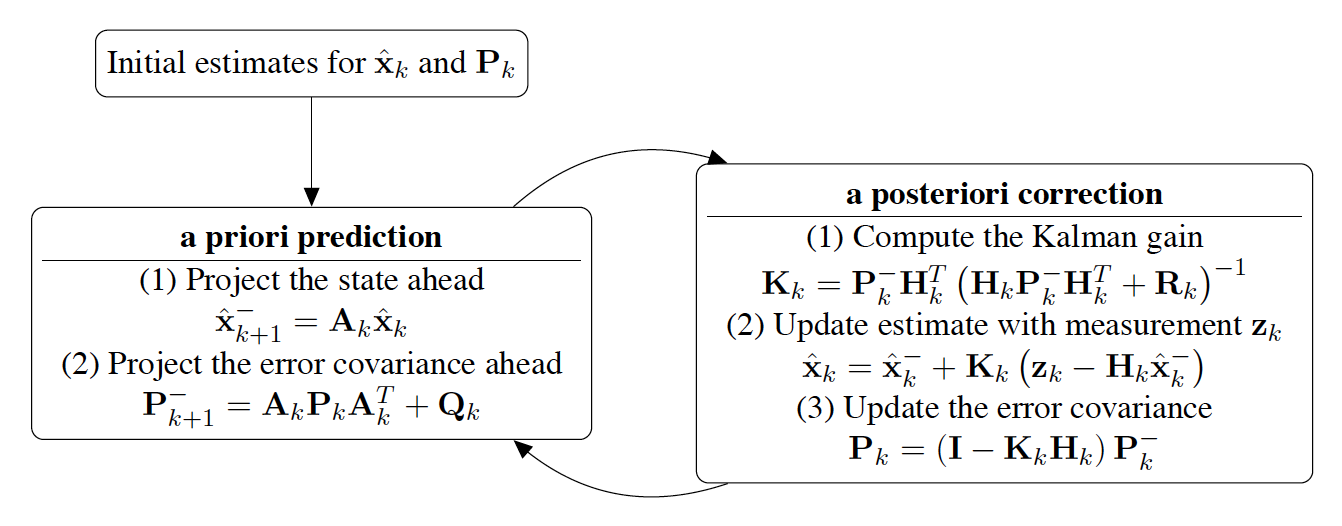
\includegraphics[width=1\linewidth]{images/kalman_scheme.png}}
	\caption{Схема работы фильтра Калмана}
	\label{fig:kalman_scheme}
\end{figure}

\subsection{Расширенный фильтр Калмана}

Для оценки нелинейных систем существует несколько расширенных версий фильтра Калмана. Широко используется подход, когда динамика системы линеаризуется вокруг априорной оценки состояния на каждом шаге по времени, а дальше с системой работают как с линейной. Этот подход известен как расширенный фильр Калмана. Стохастические уравнения~$\eqref{eq:kalman_state_evolution}$~и~$\eqref{eq:kalman_measurement}$ обобщаются на нелинейный случай.

\begin{align*}
	x_{k+1} &= f(x_k,w_k) \\
	z_k &= h(x_k,v_k)
\end{align*}

Опять же $x_k \in R^n$ - состояние, а $z_k \in R^m$ - измерение. Получим якобианы функций $f$ и $g$ (уравнения~$\eqref{eq:ext_kalman_jacob}$).

\begin{subequations}
	\begin{align}
		\label{eq:ext_kalman_A} A_{lin,k} &= \left.\left( \frac{\partial f(x_k,w_k)}{\partial x_k} \right)^T\right|_{\hat x_k^-} \\
		\label{eq:ext_kalman_W} W_{lin,k} &= \left.\left( \frac{\partial f(x_k,w_k)}{\partial w_k} \right)^T\right|_{\hat x_k^-} \\
		\label{eq:ext_kalman_H} H_{lin,k} &= \left.\left( \frac{\partial h(x_k,v_k)}{\partial x_k} \right)^T\right|_{\hat x_k^-} \\
		\label{eq:ext_kalman_V} V_{lin,k} &= \left.\left( \frac{\partial h(x_k,v_k)}{\partial v_k} \right)^T\right|_{\hat x_k^-} \\
	\notag
	\end{align}
\end{subequations}


Расширенный фильтр Калмана реализуется как показано на рис.~$\ref{fig:ext_kalman}$.

\begin{figure}
	\center{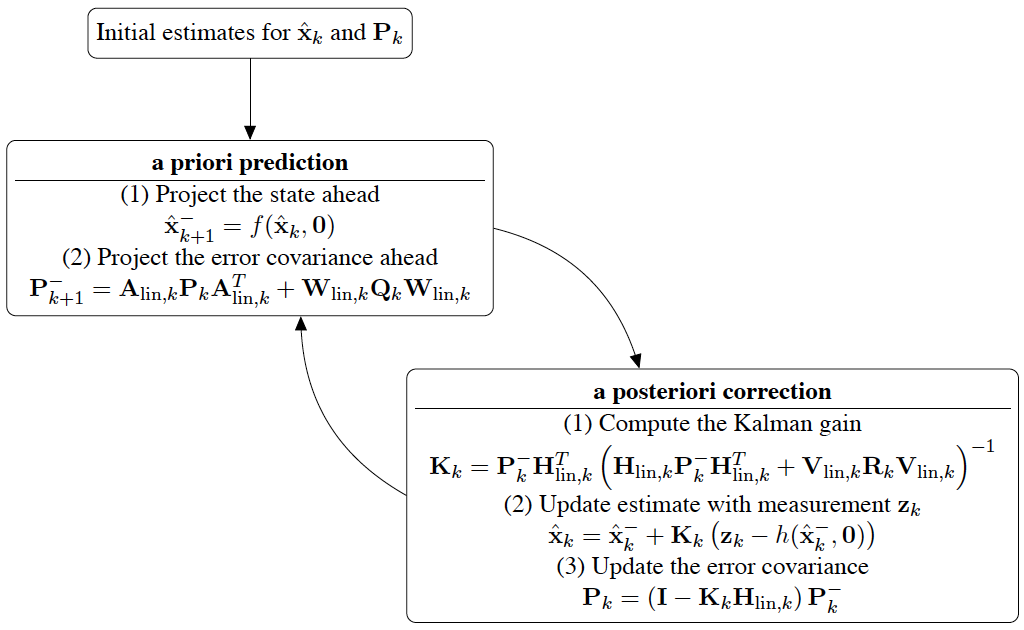
\includegraphics[width=1\linewidth]{images/ext_kalman.png}}
	\caption{Схема работы расширенного фильтра Калмана}
	\label{fig:ext_kalman}
\end{figure}


\subsection{Применение}

Расширенный фильтр Калмана применяется для оценки ориентации твердого тела в модуле  (ссылка на исходный код на гитхабе).

Вводятся две системы коородинат: BODY, связанная с телом, и NED(North East Down) - неподвижная система координат.
Вектор состояния и измерений выглядят следующим образом:

\begin{equation*}
	x = 
	\begin{vmatrix}
		{\vphantom \omega}_B \omega_{IB} \\
		{\vphantom \omega}_B \dot{\omega}_{IB} \\
		{\vphantom r}_B r_g \\
		{\vphantom r}_B r_m \\
	\end{vmatrix}, \ \
	z = 
	\begin{vmatrix}
		{\vphantom \omega}_B \bar{\omega}_{IB} \\
		{\vphantom r}_B \bar{r}_g \\
		{\vphantom r}_B \bar{r}_m \\
	\end{vmatrix}, 
\end{equation*}

где ${\vphantom \omega}_B \omega_{IB} = [\omega_x, \omega_y, \omega_z]^T$ -- угловая скорость вращения доски (вращение BODY относительно NED, измеренное в BODY), ${\vphantom \omega}_B \dot{\omega}_{IB} = [\dot\omega_x, \dot\omega_y, \dot\omega_z]^T$ -- оценка углового ускорения доски, ${\vphantom r}_B r_g = [{\vphantom r}_B r_{g,x}, {\vphantom r}_B r_{g,y}, {\vphantom r}_B r_{g,z}]^T$ -- вектор гравитации в BODY и ${\vphantom r}_B r_m = [{\vphantom r}_B r_{m,x}, {\vphantom r}_B r_{m,y}, {\vphantom r}_B r_{m,z}]^T$ -- вектор магнитного поля Земли в BODY. Нам доступны измерения вектора угловой скорости ${\vphantom \omega}_B \bar{\omega}_{IB}$ из гироскопа, вектора гравитации ${\vphantom r}_B \bar{r}_g$ из акселерометра и вектора магнитного поля ${\vphantom r}_B \bar{r}_m $ из магнитометра.

\subsubsection{Этап экстраполяции}

Полагая, что угловое ускорение не изменяется в течение $\Delta t$ между шагами, угловую скорость ${\vphantom \omega}_B \omega_{IB}$ на шаге $k+1$ легко экстраполировать из $\omega_{k+1} = \omega_k + \dot\omega_k \Delta t$. Экстраполяция двух векторных полей может быть получена похожим образом: $r_{k+1} = r_k + v_k \Delta t$. Разница в том, что мы не измеряем ${\vphantom v}_B \bar{v}_{g,k}$ и ${\vphantom v}_B \bar{v}_{m,k}$, но можем их выразить из

$$ {\vphantom v}_I v = \frac{d}{dt} {\vphantom r}_I r $$

\begin{align*}
	{\vphantom v}_B v &= A_{BI} \frac{d}{dt} {\vphantom r}_I r \\
	&= A_{BI} \frac{d}{dt} A_{IB} {\vphantom r}_B r \\
	&= \underbrace{A_{BI}A_{IB}}_I {\vphantom r}_B \dot r + \underbrace{A_{BI}\dot A_{IB}}_{{\vphantom \omega}_B \tilde\omega_{IB}} {\vphantom r}_B r \\
	&= {\vphantom r}_B \dot r +  {\vphantom \omega}_B \tilde\omega_{IB} {\vphantom r}_B r 
\end{align*}

Так как для гравитационного и магнитного полей поступательные скорости не имеют значения, мы принимаем в расчет только вращательный член $\tilde\omega_{IB} {\vphantom r}_B r$. Следовательно, нелинейная динамика системы описывается

\begin{align*}
	x_{k+1}^- = f(x_k,w_k) = 
	\begin{pmatrix}
		\omega_k + \dot\omega_k\Delta t + w_{\omega,k} \\
		\dot\omega_k + w_{\dot\omega,k} \\
		r_{a,k} + \tilde\omega_k r_{a,k} + w_{r_a,k} \\
		r_{m,k} + \tilde\omega_k r_{m,k} + w_{r_m,k} \\
	\end{pmatrix}
\end{align*}

Рассчитаем необходимые нам для этапа экстраполяции (см.~рис.~$\ref{fig:ext_kalman}$) матрицы $A_{lin,k}$, $W_{lin,k}$, как показано в $\eqref{eq:ext_kalman_A}$,~$\eqref{eq:ext_kalman_W}$.

\begin{equation*}
	A_{lin,k} = \left. \frac{\partial f(x_k,w_k)}{dx_k} \right|_{\hat x_k^-} = 
	\begin{bmatrix}
		I & I\Delta t & 0 & 0 \\
		0 & I & 0 & 0 \\
		-\tilde r_{a,k}\Delta t & 0 & I + \tilde \omega_k \Delta t & 0 \\
		-\tilde r_{m,k}\Delta t & 0 & 0 & I + \tilde \omega_k \Delta t \\
	\end{bmatrix}
\end{equation*}

\begin{equation*}
	W_{lin,k} = \left. \frac{\partial f(x_k,w_k)}{dw_k} \right|_{\hat x_k^-} = 
	\begin{bmatrix}
		I & 0 & 0 & 0 \\
		0 & I & 0 & 0 \\
		0 & 0 & I & 0 \\
		0 & 0 & 0 & I \\
	\end{bmatrix}
\end{equation*}

В этом случае этап экстраполяции для состояния выглядит

$$ \hat x_{k+1}^- = f(\hat x_k,0) $$

с опущенным шумом процесса $w$, и

$$ P_{k+1}^- = A_{lin,k}P_k A_{lin,k}^T + Q_k,$$

где на диагонали матрицы шума процесса $Q_k$ находятся дисперсии $\sigma^2$ элементов вектора состояния. Они представляют собой неопределенность предсказания. Так как эти дисперсии неизвестны и не могут быть измерены, они выступают в качестве настраиваемых параметров фильтра.


\subsubsection{Этап коррекции}

В отличие от экстраполяции состояния, измерение системы может быть описано тривиальными линейными функциями.

\begin{equation}
	\label{eq:ext_kalman_meas_impl}
	z_k = \underbrace{
		\begin{bmatrix}
			I & 0 & 0 & 0 \\
			0 & 0 & I & 0 \\
			0 & 0 & 0 & I \\
		\end{bmatrix}
	}_H
	x_k + \underbrace{
		\begin{pmatrix}
			\sigma_{\bar\omega}^2 \\
			\sigma_{\bar r_a}^2 \\
			\sigma_{\bar r_m}^2 \\
		\end{pmatrix}
	}_{R_k}.
\end{equation}

Таким образом линеаризованная матрица измерений уже дана, а якобиан из уравнения~$\eqref{eq:ext_kalman_V}$, линеаризующий влияние шума измерений $R$, вырождается в единичную матрицу $I$. Этап коррекции с рис.~$\ref{fig:ext_kalman}$ реализуется функциями для коэффициента Калмана

\begin{equation}
\label{eq:ext_kalman_K}
	K_k = P_k^- H_k^T \left(H_k P_k^- H_k^T + R_k\right)^{-1},
\end{equation}

апостериорной оценкой состояния

\begin{equation}
\label{eq:ext_kalman_x_apost}
	\hat x_k = \hat x_k^- + K_k(z_k - H_k \hat x_k^-)
\end{equation}

и апостериорной ковариацией ошибки

\begin{equation}
\label{eq:ext_kalman_P_apost}
	P_k = (I - K_kH_k)P_k^- .
\end{equation}

Для первой итерации должны быть выбраны значения a posteriori. Оценка состояния инициализируется измерениями

\begin{equation*}
	\hat x_{k,init} = 
	\begin{bmatrix}
		{\vphantom \omega}_B \omega_{IB} \\
		{\vphantom \omega}_B \dot\omega_{IB} \\
		{\vphantom r}_B r_a \\
		{\vphantom r}_B r_m \\
	\end{bmatrix}_{k,init} =
	\begin{bmatrix}
		{\vphantom \omega}_B \bar\omega_{IB} \\
		0 \\
		{\vphantom r}_B \bar r_a \\
		{\vphantom r}_B \bar r_m \\
	\end{bmatrix}_{k,init} .
\end{equation*}

А первая ковариация ошибки инициализируется значением $P_{k,init}=100I$. С течением времени, выбранное начальное значение не имеет значения, т.к. оно сходится, если инициализировано не нулем.

\subsubsection{Неполные измерения}

Так как все три трехосевых датчика (гироскоп, акселерометр, магнитометр) выдают измерения с независимыми частотами дискретизации, вектор измерений из уравнения~$eqref{ext_kalman_meas_impl}$, не всегда будет полностью доступен. Чтобы избежать использования одних и тех же измерений несколько раз, мы варьируем размер матрицы измерений $H_k$ и матрицы шума измерений $R_k$, в зависимости от того, какой датчик предоставил новые данные. В случае, когда новые данные есть у всех трех сенсоров, вектора выглядят как в уравнении~$\eqref{eq:ext_kalman_meas_impl}$. Так как гироскоп обладает наибольшей частотой дискретизации и дает ключевые данные для оценки углового ускорения $\dot\omega$, вычисления этапа коррекции будут выполняться каждый раз, когда будет доступно новое измерение $\bar \omega$. Для неполного измерения матрицы выглядят следующим образом

\begin{equation*}
	z_k = \underbrace{
		\begin{bmatrix}
			I & 0 & 0 & 0 \\
		\end{bmatrix}
	}_H + \underbrace{
		\begin{pmatrix}
			\sigma_{\bar\omega}^2 \\
		\end{pmatrix}
	}_{R_k},
\end{equation*}	

если доступны данные только от гироскопа, 

\begin{equation*}
	z_k = \underbrace{
		\begin{bmatrix}
			I & 0 & 0 & 0 \\
			0 & 0 & I & 0 \\
		\end{bmatrix}
	}_H + \underbrace{
		\begin{pmatrix}
			\sigma_{\bar\omega}^2 \\
			\sigma_{\bar r_a}^2 \\
		\end{pmatrix}
	}_{R_k},
\end{equation*}	

если доступны данные от гироскопа и акселерометра и

\begin{equation*}
	z_k = \underbrace{
		\begin{bmatrix}
			I & 0 & 0 & 0 \\
			0 & 0 & 0 & I \\
		\end{bmatrix}
	}_H + \underbrace{
		\begin{pmatrix}
			\sigma_{\bar\omega}^2 \\
			\sigma_{\bar r_m}^2 \\
		\end{pmatrix}
	}_{R_k},
\end{equation*}	

в случае данных от гироскопа и магнитометра. Весь оставшийся формализм $\eqref{eq:ext_kalman_K}$-$\eqref{eq:ext_kalman_P_apost}$ выглядит точно также. Следовательно, только те элементы вектора состояния, для которых есть новые данные от датчиков, будут корректироваться.

\subsubsection{Получение ориентации}

На каждой итерации фильтра Калмана мы оцениваем угловую скорость ${\vphantom \omega}_B \omega_{IB}$ и угловое ускорение ${\vphantom \omega}_B \dot\omega_{IB}$, но не меньший интерес представляет ориентация, которую еще нужно извлечь. Чтобы избежать проблем с сингулярностью, мы представляем ориентацию матрицей поворота $3 \times 3$ $A_{BI}$. Этого можно достичь с помощью описания трех единичных базисных векторов начальной системы координат в системе координат связанной с телом. 

$$ A_{BI} = 
	\begin{bmatrix} 
		{\vphantom e}_B e_{I_x} & {\vphantom e}_B e_{I_y} & {\vphantom e}_B e_{I_z} \\
	\end{bmatrix}
$$

Три базовых вектора извлекаются из оценок вектора ускорения ${\vphantom r}_B \hat r_a$ и вектора магнитного поля ${\vphantom r}_B \hat r_m$. Заметим, что в качестве инерциальной системы координат используется система координат NED (North-East-Down). Как упоминалось выше, опуская поступательное ускорение доски в сравнении с гравитацией, базисный вектор в направлении оси $z$ можно записать в виде

$$ {\vphantom e}_B e_{I_z} = -\frac{{\vphantom r}_B r_a}{\|{\vphantom r}_B r_a\|}_2 .$$

Вдобавок, инерциальную систему координат всегда можно выбрать таким образом, чтобы базисный вектор $x$ соответствовал магнитному полю Земли. Однако, так как измерение никогда не будет точным, мы не используем этот вектор прямым образом для получения ${\vphantom r}_B r_{I_x}$, а используем, сохраняя ортогональность инерциальной системы, для расчета базисного вектора в направлении $y$

$$ {\vphantom e}_B e_{I_y} = \frac{{\vphantom e}_B e_{I_z} \times {\vphantom r}_B r_m}{\| {\vphantom e}_B e_{I_z} \times {\vphantom r}_B r_m\|_2} .$$

Определены два вектора, третий всегда может быть вычислен из ортогональности системы координат:

$$ {\vphantom e}_B e_{I_x} = \frac{{\vphantom e}_B e_{I_y} \times {\vphantom e}_B e_{I_z}}
	{\| {\vphantom e}_B e_{I_y} \times {\vphantom e}_B e_{I_z} \|_2} .$$

\section{Оценка из простейшей физики и геометрии}

\begin{figure}
	\centering
	\begin{tikzpicture}
		\draw[thick] (-2.5,0) arc (180:360:2.5cm);
		\node[below left] at (-2.5,0) {$-R$};
		\node[below right] at (2.5,0) {$R$};

		\draw[thick] (-2.5,0) -- (2.5,0);
		\draw[thick] (-1,0) rectangle (1,4);
		\node[above right] at (0,4) {$h$};
		\node[below] at (-1,0) {$-w/2$};
		\node[below] at (1,0) {$w/2$};

		\draw[thick,dashed] (-2.7,-1) -- (2.7,-1);
		\node[below right] at (0,-1) {$d$};
		%\draw[step=1cm,gray,very thin] (-3.5,-3.9) grid (3.5,5.9);
		\draw[thick,->] (-3.4,0) -- (3.4,0) node[anchor=north west] {$x$};
		\draw[thick,->] (0,-3.4) -- (0,5.8) node[anchor=south east] {$y$};

		\node[below right] at (0,0) {0};
	\end{tikzpicture}
	\caption{Модель полукруглой доски и параллелепипедного груза}	
	\label{fig:simple_model}
\end{figure}

Мы рассмотрим фактически плоскую модель, основанную на законе изменения момента импульса. Для более сложных моделей обратитесь к \cite{fossen_marine_control}.

В плоской модели (cм.~рис.~$\ref{fig:simple_model}$) доска характеризуется ее поперечным сечением и на протяжении всей длины выглядит одинаково. Груз точно также характеризуется своим сечением хоть и может быть другой длины. Единственное требование состоит в том, что центры масс доски и груза лежат на одной длине (имеется в виду длина вглубь картинки). Доска имеет полукруглое сечение, а груз прямоугольное.

\subsection{Центр масс}

Сила тяжести приложена в центре масс, поэтому первым делом найдем его координаты.

Центр масс груза найти просто: это точка $(0, h/2)$.

Центр масс лодки:

\begin{align*}
	x_c & = 0 \\
	y_c & = \frac{\int\limits_0^R \int\limits_0^{-\pi} r^2 \sin \varphi dr d\varphi}{\pi R^2/2} 
		= \frac{\int\limits_0^R r^2 dr \int\limits_0^{-\pi}  \sin \varphi d\varphi}{\pi R^2/2} \\
		& = \frac{2R^3/3}{\pi R^2/2} = \frac{4R}{3\pi} 
\end{align*}

Итого, центр масс всего объекта - $(0, \frac{m_\text{г}h/2 + m_\text{л}4R /3\pi }{m_\text{г} + m_\text{л}})$

\subsection{Центр плавучести от угла наклона}

В центре плавучести приложена сила Архимеда, поэтому нам важно знать его положение для оценки плеча.

\subsubsection{Глубина погружения}
Для начала найдем глубину, на которую погружается лодка в начальном положении. Запишем условие равновесия.

$$ (m_\text{г} + m_\text{л})g = F_A = \rho_\text{в}gLS_0, $$

где $S_0$ - площадь подводной части в положении равновесия.

$$ S_0 = \frac{m_\text{г} + m_\text{л}}{\rho_\text{в}L} $$

\begin{figure}
	\centering
	\begin{tikzpicture}
		\draw[thick] (-1.5,0) arc (180:360:1.5cm);
		\draw[thick] (-1.5,0) -- (1.5,0);
		\draw[thick,dashed] (-1.7, -0.5) -- (1.7, -0.5);
		\draw[thick,dashed] (-1.7, 0) -- (-1.5, 0);
		\draw[thick,dashed] (1.5, 0) -- (1.7, 0);
		\draw[<->] (-0.2, -0.5) -- (-0.2, 0);
		\node[below] at (0, 0) {$d$};
		\node[above] at (0, -1.3) {$S_0$};
		\node[above] at (0.75, 0) {$R$};
	\end{tikzpicture}
	\caption{Оценка ватерлинии}	
	\label{fig:waterline}
\end{figure}

Дальше решаем геометрическую задачу, в которой известен радиус круга и площадь сегмента, а найти требуется расстояние между диаметром параллельным хорде и самой хордой.

Полукруг состоит из заданного сегмента, прямоугольника и двух маленьких плавников. Рассмотрим приближение, в котором площадь плавников мала.

$$ \frac{\pi R^2}{2} = S_0 + d\sqrt{R^2-d^2} $$
$$ d^2(R^2-d^2) = \frac{1}{4}(\frac{\pi R^2}{2} - S_0)^2 $$

Обозначим правую часть за $C$

$$ d^4 - R^2d^2 + C = 0 $$
$$ t^2 - R^2t + C = 0 $$
$$ t = \frac{R^2 \pm \sqrt{R^4-4C}}{2} $$

Из соображений соразмерности и того, что $d$ должен уменьшаться с увеличением $S_0$ оставляем только знак минус.

$$ d = \sqrt{\frac{R^2 - \sqrt{R^4-4C}}{2}} $$
$$ d = \sqrt{\frac{R^2 - \sqrt{R^4-(\frac{\pi R^2}{2} - S_0)^2}}{2}} $$

Если $d$ много меньше $R$ то площадь плавников стремиться к нулю. Насколько верно это соотношение надо судить из опыта.

\subsubsection{Площадь подводной части}

Для разминки вычислим площадь подводной части в начальном положении, используя найденное расстояние $d$. 

Вычислим следующий вспомогательный интеграл:
$$ I_{ab} = \int\limits_a^b \sqrt{\lambda^2 - x^2}\;dx $$

\begin{align*}
	I_{ab} &= \lambda^2 \int\limits_\frac{a}{\lambda}^\frac{b}{\lambda} \sqrt{1 - t^2}\;dt 
	= \lambda^2 \int\limits_\frac{a}{\lambda}^\frac{b}{\lambda} \frac{1 - t^2}{\sqrt{1 - t^2}}\;dt \\
	&= \lambda^2 \int\limits_{\arcsin\frac{a}{\lambda}}^{\arcsin\frac{b}{\lambda}} \cos^2u\;du 
	= \lambda^2 \int\limits_{\arcsin\frac{a}{\lambda}}^{\arcsin\frac{b}{\lambda}} \frac{1-\cos2u}{2}\;du \\
	&= \frac{\lambda^2}{2}(\arcsin\frac{b}{\lambda} - \arcsin\frac{a}{\lambda}) - \frac{\lambda^2}{4}(\sin 2\arcsin\frac{a}{\lambda} - \sin 2\arcsin\frac{b}{\lambda}) 
\end{align*}

Начальная подводная площадь:

$$ S_b = \int_{x_1}^{x_2} \int_{-\sqrt{R^2-x^2}}^{-d} dx dy, $$

где $x_1$, $x_2$ - точки пересечения полукруга и прямой $y=-d$. 

$$ x_2 = -x_1 = \hat{x} =\sqrt{R^2 - d^2} $$

$$ S_b = \int_{-\hat{x}}^{\hat{x}} \int_{-\sqrt{R^2-x^2}}^{-d} dx dy $$
$$ S_b = \int_{-\hat{x}}^{\hat{x}} \sqrt{R^2-x^2} dx - 2d\hat{x} $$

$$ S_b = R^2 \arcsin\frac{\hat{x}}{R} + \hat{x}R\cos\arcsin\frac{\hat{x}}{R} - 2d\hat{x} $$

Косинус угла, синус которого равен $\frac{\hat{x}}{R}$, равен $\frac{d}{R}$. Поэтому

$$ S_b = R^2 \arcsin\frac{\hat{x}}{R} + \hat{x}R\cos\arccos\frac{d}{R} - 2d\hat{x} $$
$$ S_b = R^2 \arcsin\frac{\hat{x}}{R} + \hat{x}d - 2d\hat{x} $$
$$ S_b = R^2 \arcsin\frac{\hat{x}}{R} - d\hat{x} $$
$$ S_b = R^2 \arcsin\frac{\sqrt{R^2-d^2}}{R} - d\sqrt{R^2-d^2} $$

Теперь найдем центр масс сегмента.

$$ y_s = \int_{-\hat{x}}^{\hat{x}} \int_{-\sqrt{R^2-x^2}}^{-d} y dx dy $$
$$ y_s = \frac{1}{2} \int_{-\hat{x}}^{\hat{x}} d^2 - R^2 + x^2 dx $$
$$ y_s = (d^2 - R^2)\sqrt{R^2-d^2}  $$

В ординате центра плавучести в начальном положении нас интересует не сама координата, а расстояние от центра круга до центра плавучести. В данном случае оно совпадает с ординатой.

Чтобы получить зависимости этих двух величин от угла наклона, посмотрим на наклон немного с другой стороны. Мы уже умеем находить площадь сегмента зная расстояние между его хордой и диаметром. После поворота нам тоже нужно найти площадь сегмента, только расстояние до хорды поменяется с $d$ на $d\cos\alpha$. 

Следовательно, 

$$ S_b(\alpha) = R^2 \arcsin\frac{\sqrt{R^2-d^2\cos^2\alpha}}{R} - d\cos\alpha\sqrt{R^2-d^2\cos^2\alpha} $$

$$ y_s(\alpha) = (R^2-d^2\cos^2\alpha)^{\frac{3}{2}} $$


\subsection{Моменты действующих сил}

На лодку с грузом действуют две силы: сила тяжести и сила Архимеда. Сила тяжести приложена в центре масс, а сила Архимеда - в центре плавучести. 

Ось, вокруг которой вращается лодка, находится на уровне жидкости в начальном положении. Если принять этот уровень за $-d$, то ось представляет собой прямую, направленную по оси $z$ вглубь лодки и имеющую координаты $(0, -d)$.

При отклонении на угол $\alpha$. Плечо силы тяжести будет равно $(y_c+d)\sin\alpha$, а момент, соответсвенно:

$$ M_{mg} = (m_\text{г} + m_\text{л})g (\frac{m_\text{г}\frac{h}{2} + m_\text{л}\frac{4R}{3\pi}}{m_\text{г} + m_\text{л}} + d) \sin\alpha = (m_\text{г}\frac{h}{2} + m_\text{л}\frac{4R}{3\pi} + (m_\text{г} + m_\text{л})d)g\sin\alpha $$

Вообще говоря, нам не так важно само расстояние от центра круга до центра плавучести, сколько важен факт, что они лежат на прямой перпендикулярной уровню воды. Отсюда следует, что плечо силы Архимеда равно $d\sin\alpha$.

$$ M_A = \rho_\text{в}gLS_b(\alpha)d\sin\alpha $$

$$ M_A = \rho_\text{в}gLd\sin\alpha (R^2 \arcsin\frac{\sqrt{R^2-d^2\cos^2\alpha}}{R} - d\cos\alpha\sqrt{R^2-d^2\cos^2\alpha}) $$

\subsection{Момент инерции}

Момент инерции параллелепипеда вычисляется просто:

$$ I_p = \frac{m}{12}(w^2 + h^2) + m(d + \frac{h}{2})^2 $$

С полукругом сложнее, придется снова возится с интегралами:

$$ I_{hs} = \int_0^L \int_{-R}^{R} \int_{-\sqrt{R^2 - x^2}}^0 (x^2 + (y-d)^2) dx dy dz $$
$$ I_{hs} = L \int_{-R}^{R} \int_{-\sqrt{R^2 - x^2}}^0 (x^2 + y^2 -2yd + d^2) dx dy $$
$$ I_{hs} = L \int_{-R}^{R} (x^2 \sqrt{R^2 - x^2} + (R^2 - x^2)^\frac{3}{2} - d(R^2 - x^2) + d^2 \sqrt{R^2 - x^2}) dx $$

$$ I_{hs} = L \int_{-R}^{R} (x^2 \sqrt{R^2 - x^2} + (R^2 - x^2)^\frac{3}{2}) dx - 2LdR^3 + Ld\frac{2R^3}{3} + Ld^2\pi\frac{R^2}{2} $$

$$ I_{hs} = L\pi\frac{R^4}{8} + L\pi\frac{3R^4}{8} - Ld\frac{4R^3}{3} + Ld^2\pi\frac{R^2}{2} $$

$$ I_{hs} = \frac{\pi LR^4}{2} + \frac{\pi Ld^2R^2}{2} - \frac{4LdR^3}{3} $$

Этот интеграл еще умножается на плотность. Но мы лучше выразим все через массу, т.к. известен объем лодки $\frac{\pi LR^2}{2}$.

$$ I_{hs} = mR^2 + md^2 - \frac{8mdR}{3\pi}$$

Так как момент инерции это аддитивная величина, то суммарный момент лодки и груза будет равен:

$$ I = \frac{m_\text{г}}{12}(w^2 + h^2) + m_\text{г}(d + \frac{h}{2})^2 + m_\text{л}R^2 + m_\text{л}d^2 - \frac{8m_\text{л}dR}{3\pi}$$

\subsection{Уравнение движения}

Уравнение движения мы получим из закона изменения момента импульса $\dot{L} = M$. В нашем случае это выглядит следующим образом:

$$ I\dot{\omega} = M_{mg} - M_A $$

$$ (\frac{m_\text{г}}{12}(w^2 + h^2) + m_\text{г}(d + \frac{h}{2})^2 + m_\text{л}R^2 + m_\text{л}d^2 - \frac{8m_\text{л}dR}{3\pi})\ddot{\alpha} = $$
$$ = (m_\text{г}\frac{h}{2} + m_\text{л}\frac{4R}{3\pi} + (m_\text{г} + m_\text{л})d)g\sin\alpha -  \rho_\text{в}gLd\sin\alpha (R^2 \arcsin\frac{\sqrt{R^2-d^2\cos^2\alpha}}{R} - d\cos\alpha\sqrt{R^2-d^2\cos^2\alpha}) $$


\section{Идентификация}

Вывод моделей из наблюдений и изучение свойств этих моделей -- это и есть наука. Модели (<<гипотезы>>, <<законы природы>>, <<парадигмы>> и т.п.) могут иметь более или менее формальных характер, но одно основное свойство у них общее: они пытаются связать наблюдения в некую схему. Задача идентификации состоит в построении математических моделей динамических систем, основыванном на наблюдении.

Построение модели из данных включает в себя три базовых элемента:

\begin{enumerate}
	\item Данные
	\item Набор моделей-кандидатов
	\item Правило, по которому модели кандидаты могут быть оценены с использованием данных
\end{enumerate}

Прокомментируем каждый пункт подробнее:

\begin{enumerate}
	\item \textit{Запись данных}. Иногда входные/выходные данные записываются во время специально организованного эксперимента, в котором пользователь определяет какие сигналы измерять и когда их измерять, а также может выбирать входные сигналы. Эксперимент обычно организовывается таким образом, чтобы записываемые сигналы были максимально информативными. В других случаях у пользователя нет возможности влиять на эксперимент, но он может использовать данные нормального функционирования системы.

	\item \textit{Набор моделей}. Выбор моделей -- несомненно самый важный и, в то же время, самый сложный выбор в процедуре идентификации. Это то место, где априорные знания и инженерная интуиция комбинируются с формальными параметрами моделей. Иногда набор моделей получают внимательным моделированием. В этом случае модель с некоторыми неизвестными физическими параметрами строится из базовых физических законов и других установленных соотношений. В других случаях используются стандартные линейные модели без физической подоплеки.

	\item \textit{Определение <<лучшей>> модели из набора (руководствуясь снятыми данными)}. Это \textit{метод идентификации}. Оценка качества модели обычно основывается на том, как ведут себя модели в попытке воспроизвести измеренные данные.
\end{enumerate}

Подробнее о задаче идентификации и способах ее решения можно прочитать в \cite{ljung_identification}


\subsection{Из экспериментов}


\subsubsection{Моторы и винты}

Ни для кого не секрет, что вращаясь, гребные винты толкают корабли вперед, т.е. дают тягу. Но еще больше ста лет назад Жуковский изучал зависимость тяги винта от скорости его вращения. Так как входным сигналом для плавательной доски является тяга, то мы тоже должны были изучить этот вопрос (хотя бы примерно). 

\begin{figure}[h]
	\center{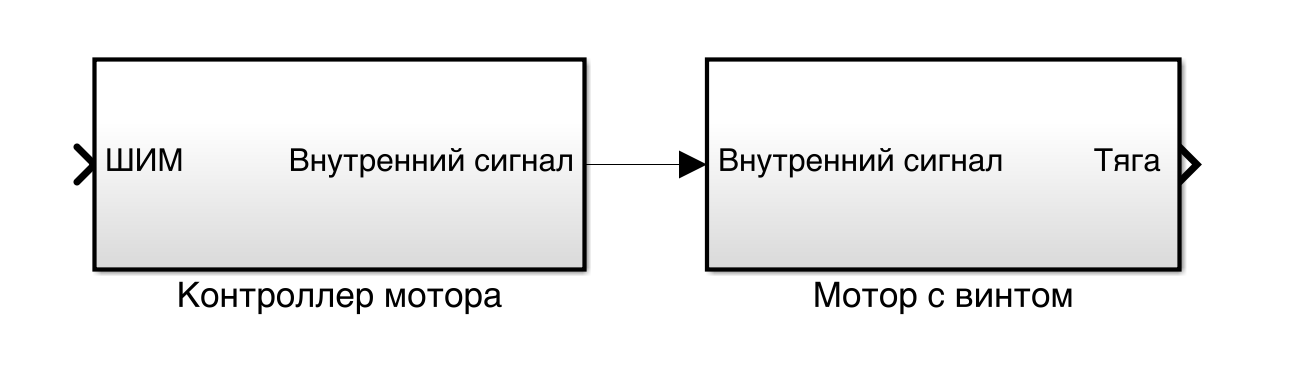
\includegraphics[width=1\linewidth]{images/propeller_research.png}}
	\caption{Схема управления тягой связки мотор-винт}
\end{figure}

Проблема еще состоит в том, что контроллеры управления моторами не позволяют управлять оборотами напрямую. В наших возможностях изменение скважности широтно-импульсно-модулированного сигнала. 

\begin{figure}[h]
	\center{\includegraphics[width=1\linewidth]{images/propeller_research_installation.png}}
	\caption{Установка для оценки зависимости тяги от шима}
\end{figure}

Эксперимент предельно прост:

\begin{enumerate}
	\item Подключаем управляющую электронику и надеваем винт на мотор
	\item Подавая различные управляющие сигнал меряем тягу с помощью безмена (на фотографии голубой)
	\item Замеряем отношение плечей рычага (0.29)
\end{enumerate}

В результате мы имеем:

\begin{table}[h]
	\caption{Зависимость тяги от скважности ШИМа}
	\label{thrust_on_pwm_data}
	\begin{center}
		\begin{tabular}{cccccc}
			Управляющий сигнал &  Тяга 1 & Тяга 2 & Тяга 3 & Средняя & Приведенная \\
			-0.90 & 0.06 & 0.05 & 0.08 & 0.063 & 0.01837 \\
			-0.85 & 0.08 & 0.1 & 0.11 & 0.097 & 0.028 \\
			-0.80 & 0.145 & 0.18 & 0.215 & 0.18 & 0.0522 \\
			-0.75 & 0.235 & 0.28 & 0.26 & 0.258 & 0.0749 \\
			-0.70 & 0.29 & 0.32 & 0.325 & 0.312 & 0.09 \\
			-0.65 & 0.32 & 0.34 & 0.415 & 0.358 & 0.104 \\
			-0.60 & 0.475 & 0.44 & 0.465 & 0.46 & 0.1334 \\
			-0.55 & 0.54 & 0.525 & 0.55 & 0.538 & 0.156 \\
			-0.50 & 0.67 & 0.62 & 0.625 & 0.638 & 0.185 \\
			-0.45 & 0.735 & 0.7 & 0.74 & 0.725 & 0.21 \\
			-0.40 & 0.9 & 0.92 & 0.89 & 0.903 & 0.262 \\
		\end{tabular}
	\end{center}
\end{table}

Кривая $\ref{thrust_on_pwm_plot}$, в принципе, похожа на параболу, но для нашей точности хватит и прямой на этом участке.

\begin{figure}[h]
	\center{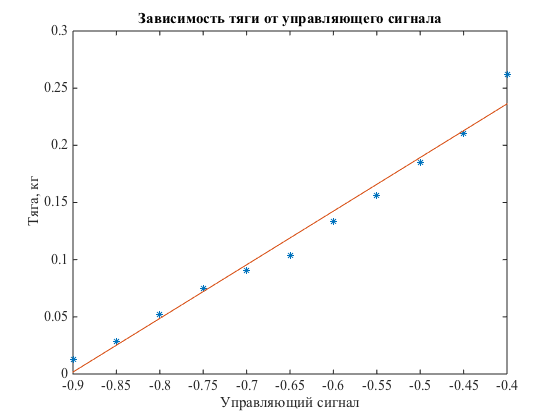
\includegraphics[width=1\linewidth]{images/thrust_on_pwm_plot.png}}
	\caption{Аппроксимация прямой зависимости тяги от шима}
	\label{thrust_on_pwm_plot}
\end{figure}

Таким образом, если обозначить за $c$ - управляющий сигнал, а за $F$ - тягу, то зависимость имеет вид

$$ F = 0.4691c + 0.4239 $$


\subsubsection{Маятник}

Если считать лодку маятником, то ее передаточная функция

$$ H_{pend} = \frac{1}{s^2 + a_1s + a_0s} $$

В зависимости от наличия груза и высоты его прикрепления меняются коэффициенты $a_1$ и $a_0$.

Мотор, в этом случае, выглядит как

$$ H_{smotor} = \frac{b}{Ts+1} $$

Рассмотрим дифференциальное уравнение маятника

\begin{equation}
	\label{pend_eq}
	\ddot{x} + \frac{c}{m}\dot{x} + \frac{k}{m}x = 0, \ x(0) = x_0, \ \dot{x}(0) = 0 
\end{equation}

Его решение легко получить

$$ x(t) = x_0 \exp\left(-\frac{ct}{2m}\right) \left( \cos\frac{t\sqrt{4km-c^2}}{2m} + \frac{c}{\sqrt{4km-c^2}} \sin\frac{t\sqrt{4km-c^2}}{2m} \right) $$

Оно представляет собой колебания вокруг ноля с частотой $\frac{\sqrt{4km-c^2}}{2m}$ между двумя затухающими экспонентами: $x_0 \exp{-\frac{ct}{2m}}$ и $-x_0 \exp{-\frac{ct}{2m}}$

\begin{figure}[h]
	\center{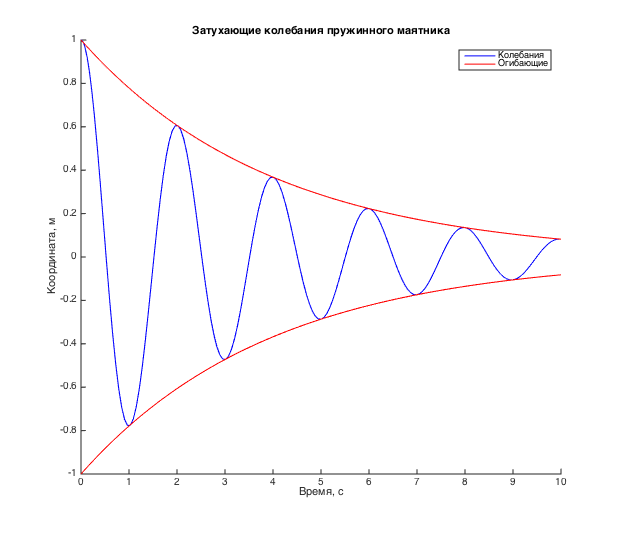
\includegraphics[width=1\linewidth]{images/pendulum_example.png}}
	\caption{Решение уравнения $\ref{pend_eq}$ с параметрами $m = 1$ кг, $c = 0.5$ кг/с, $k = 10$ Н/м, $x_0=1$ м}
\end{figure}

Отсюда вытекает первый эксперимент, который я провел. Ставим лодку на воду, отклоняем на небольшой угол и отпускаем. Все углы и угловые скорости записываются. В результате мы получаем картинку похожую на колебания пружинного маятника и, соответственно, можем оценить его параметры. Для простоты введем два параметра: $\alpha$ - показатель затухания экпоненты, и $\omega$ - частота колебаний. Запишем систему уравнений

\begin{equation*}
	\begin{cases}
		\frac{c}{2m} = \alpha
		\\
		\sqrt{\frac{k}{m} - \frac{c^2}{4m^2}} = \omega
	\end{cases}
\end{equation*}

Следовательно, 

\begin{equation*}
	\begin{cases}
		a_1 = \frac{c}{m} = 2\alpha
		\\
		a_0 = \frac{k}{m} = \omega^2 + \alpha^2
	\end{cases}
\end{equation*}

\begin{figure}[h]
	\center{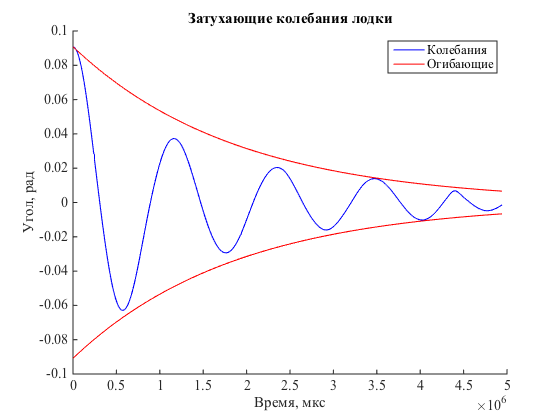
\includegraphics[width=1\linewidth]{images/pendulum_boat.png}}
	\caption{Эксперимент с отклонением лодки}
\end{figure}

Реальные данные совпадают с теоретическими неидеально, но $\alpha$ и $\omega$ оценить можно. Затухание подбираем на глаз, а частоту - замеряя промежутки между максимумами и минимумами. Ключевое здесь - не забыть про множитель $2\pi$.

\begin{table}[h]
	\caption{Параметры маятникообразных колебаний}
	\label{boat_pend_params}
	\begin{center}
		\begin{tabular}{ccc}
			$\alpha$ &  0.53 \\
			$\omega$ &  5.85 \\
		\end{tabular}
	\end{center}
\end{table}

Таким образом мы получаем коэффициенты нашей лодки приблизительно равными  (см. $\ref{pend_boat_params}$)

\begin{table}[h]
	\caption{"Маятниковые" параметры лодки}
	\label{pend_boat_params}
	\begin{center}
		\begin{tabular}{cc}
			$a_1$ &  1.06 \\
			$a_0$ &  34.5 \\
		\end{tabular}
	\end{center}
\end{table}


\subsubsection{Автоколебания}

Второй эксперимент основан на свойстве динамических систем входить в режим автоколебаний на границе устойчивости. Ввести систему в автоколебания легко: достаточно добавить пропорциональный регулятор и отрицательную обратную связь. Передаточная функция такой разомкнутой системы

$$ H_{openloop} = \frac{bk}{(Ts+1)(s^2+a_1s+a_0)} $$

Характеристический полином же

$$ P(s) = Ts^3 + (Ta_1+1)s^2 + (Ta_0+a_1)s + a_0 + bk $$

Найдем его корни в виде $s=j\omega$, где $\omega$ - угловая частота автоколебаний.

$$ P(j\omega) = -jT\omega^3 - (Ta_1+1)\omega^2 + j(Ta_0+a_1)\omega + a_0 + bk  = R(\omega) + jS(\omega) = 0$$

\begin{equation*}
	\begin{cases}
		R(\omega) = - (Ta_1+1)\omega^2 + a_0 + bk = 0
		\\
		S(\omega) = -jT\omega^3 + j(Ta_0+a_1)\omega = 0
	\end{cases}
\end{equation*}

В результате получаем еще два условия для идентификации объекта

\begin{equation*}
	\label{self_oscil_cond}
	\begin{cases}
		\omega^2 = \frac{a_0 + bk}{Ta_1 + 1}
		\\
		\omega^2 = \frac{Ta_0+a_1}{Ts}
	\end{cases}
\end{equation*}

Увеличивая пропорциональный коэффициент регулятора, находим максимальное значение, при котором лодка еще не переворачивается, т.е. не теряет устойчивости. Этого удалось достигнуть при $k = 4$. Частота автоколебаний определяется расстоянием между максимумами.

\begin{figure}[h]
	\center{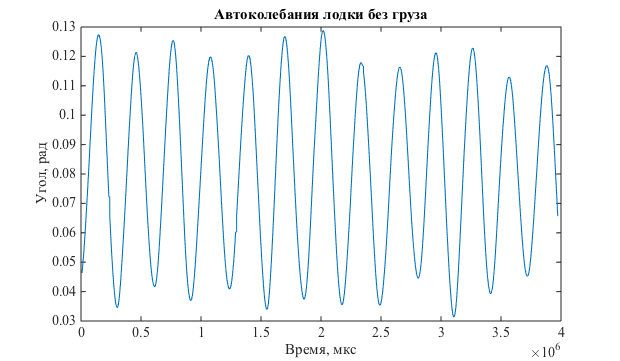
\includegraphics[width=1\linewidth]{images/self_oscil_no_cargo.png}}
	\caption{Автоколебания лодки без груза, $k = 4$}
\end{figure}

Средний период $T_{\text{ср}} = 0.311$ c

Решая систему $\ref{self_oscil_cond}$ с параметрами $\omega = 20.2$, $k = 4$, $a_0 = 34.5$, $a_1 = 1.06$, получим $T = 2.8 \cdot 10^{-3}$, $b = 93.7$.

Итого, параметры лодки без груза 

\begin{table}[h]
	\caption{Параметры лодки без груза}
	\label{table:boat_params_no_cargo}
	\begin{center}
		\begin{tabular}{cl}
			$a_1$ &  1.06 \\
			$a_0$ &  34.5 \\
			$T$ & $2.8 \cdot 10^{-3}$ \\
			$b$ & 93.7 \\
		\end{tabular}
	\end{center}
\end{table}

При добавлении груза повторяем опыт с автоколебаниями и снова решаем систему $\ref{self_oscil_cond}$, но уже относительно $a_0$ и $a_1$.

При частоте автоколебаний с грузом $\omega_{cargo} = 20.62$ и пропорциональном коэффициенте $k = 5.5$ получим

\begin{table}[h]
	\caption{Параметры лодки с грузом}
	\label{table:boat_params_cargo}
	\begin{center}
		\begin{tabular}{cl}
			$a_1$ &  2.93 \\
			$a_0$ &  -513.62 \\
			$T$ & $2.8 \cdot 10^{-3}$ \\
			$b$ & 93.7 \\
		\end{tabular}
	\end{center}
\end{table}


\section{Стабилизация}

Выпишем еще раз наш объект

$$ G = \frac{1}{Ts+1} \frac{b}{s^2+a_1s+a_0} $$

его примерные коэффициенты мы узнали из идентификационных процедур.

Рассмотрим устойчивость объекта. Одним из критериев устойчивости объекта является критерий Гурвица.

Пусть $U(s) = a_0s^n + a_1s^{n-1} + \dots + a_n $ - характеристический полином системы. Из коэффициентов характеристического уравнения строится определитель Гурвица $\Delta$ по алгоритму:

\begin{enumerate}
	\item по главной диагонали выставляем коэффициенты характеристического полинома от $a_1$ до $a_n$
	\item от каждого элемента диагонали вверх и вниз достраиваем столбцы определителя так, чтобы индексы убывали сверху вниз
	\item на место коэффициентов с индекса меньше 0 или больше $n$ cтавятся нули
\end{enumerate}

Критерий Гурвица звучит следующим образом. Для того, чтобы динамическая система была устойчива необходимо и достаточно, чтобы все $n$ главных диагональных миноров определителя Гурвица были положительны, при условии $a_0 > 0$.

Применим этот метод для полинома третьей степени. Характеристический полином:

$$ U(s) = a_0s^3 + a_1s^2 + a_2s + a_3 $$

Определитель Гурвица:

\begin{equation*}
	\Delta = 
	\begin{vmatrix}
		a_1 & a_3 & 0 \\
		a_0 & a_2 & 0 \\
		0 & a_1 & a_3 \\
	\end{vmatrix}
\end{equation*}

Условия устойчивости будут:

\begin{equation*}
	\begin{cases}
		&a_0 > 0 \\
		&a_1 > 0 \\
		&a_1a_2 > a_0a_3 \\
		&a_3 > 0 \\
	\end{cases}
\end{equation*}

В случае, когда $a_0 = T^\text{л}$, $a_1 = T^\text{л} a_1^\text{л} + 1$, $a_2 = T^\text{л} a_0^\text{л} + a_1^\text{л}$, $a_3 = a_0^\text{л}$, условия устойчивости будут выглядеть

\begin{equation*}
	\begin{cases}
		&T^\text{л} > 0 \\
		&T^\text{л}a_1^\text{л} + 1 > 0 \\
		&(T^\text{л}a_1^\text{л} + 1)(T^\text{л}a_0^\text{л} + a_1^\text{л}) > T^\text{л}a_0^\text{л} \\
		&a_0^\text{л} > 0 \\
	\end{cases}
\end{equation*}

Проверим лодку с грузом и без на устойчивость. Без груза (см. табл. $\ref{table:boat_params_no_cargo}$)

\begin{equation*}
	\begin{cases}
		&2.8 \cdot 10^{-3} > 0 \\
		&2.8 \cdot 10^{-3} \cdot 1.06 + 1 > 0 \\
		& (2.8 \cdot 10^{-3} \cdot 1.06 + 1)(2.8 \cdot 10^{-3} \cdot 34.5 + 1.06) > 2.8 \cdot 10^{-3} \cdot 34.5 \\
		&34.5 > 0 \\
	\end{cases}
\end{equation*}

Лодка без груза устойчива. Теперь с грузом (см. табл. $\ref{table:boat_params_cargo}$). Хватит и одного условия, чтобы понять, что лодка с грузом неустойчива.

$$ -513.62 < 0 $$

\cite{polyak_scherbakov_robust}

\subsection{Запасы устойчивости} 

Как измерить насколько устойчив объект? На этот вопрос проще дать ответ в терминах обратной связи.

Замкнем наш объект отрицательной обратной связью.

\begin{figure}
	\center{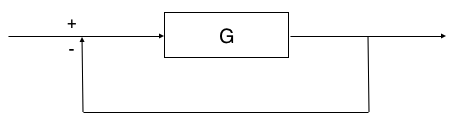
\includegraphics[width=1\linewidth]{images/closed_loop_nocontr.png}}
	\caption{Система с обратной связью}
\end{figure}

Передаточная функция такой системы будет

$$ H = \frac{G}{1+G} $$

Система будет неустойчива, если на какой-то частоте $G(jw) = -1$, так как это означает, что у системы на этой частоте бесконечный коэффициент усиления, а так как в реальных системах неизбежно присутствует шум, то природа обязательно подаст на вход сигнал на этой критической частоте. 

Если представить $G$ в виде $G = |G|\exp(j\arg G)$, то условие $G(jw) = -1$ перепишется в виде:

\begin{equation*}
	\begin{cases}
		|G| = 1 \\
		\arg G = \pi
	\end{cases}
\end{equation*}

Отсюда вытекает определение запасов устойчивости.

Если $|G(j\omega_{gc}| = 1$, то $\arg G(j\omega_{gc})$ - это запас устойчивости по фазе.

Если $\arg G(j\omega_{pc}) = \pi$, то $|G(j\omega_{pc}|$ - это запас устойчивости по амплитуде.

Обычно запас устойчивости по амплитуде измеряется в децибелах, т.е.

$$ 20 \log_{10} |G(j\omega_{pc})|, $$

а запас устойчивости по фазе - в градусах.

Эти параметры удобно вычислять либо с помощью ЛАФЧХ (в англоязычной литературе - диаграмм Боде), либо просто рисуя передаточную функцию разомкнутой системы на комплексной плоскости при различных частотах.

\subsection{D-разбиение}

Добавим в цепь регулятор и попробуем найти область коэффициентов регулятора, при которых замкнутая система устойчива.

\begin{figure}
	\center{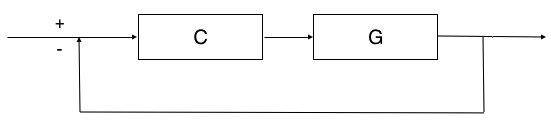
\includegraphics[width=1\linewidth]{images/closed_loop_contr.png}}
	\caption{Система с регулятором}
\end{figure}

Наш регулятор - пропорционально-дифференциальный, т.е. $C(s) = k_p + k_d s$. Область устойчивости на плоскости коэффициентов $(k_p, k_d)$ можно найти с помощью D-разбиения. Идея метода заключается в следующем. Пусть при каком либо $k = (k_p, k_d)$ степень характеристического полинома системы $P(s,k)$равна $n$ и он имеет $m \le n$ корней в левой полуплоскости и $n - m$ -- в правой. Как при изменении $k$ может измениться расположение корней? Ясно, что это может произойти только в одном из следующих случаев:

\begin{enumerate}
	\item изменится степень полинома $P(s,k)$;
	\item вещественный корень $P(s,k)$ перейдет из одной полуплоскости в другую, т.е. станет равным нулю;
	\item пара комплексных корней перейдет из одной полуплоскости в другую т.е. $P(s,k)$ будет иметь пару чисто мнимых корней $\pm j\omega$.
\end{enumerate}

Таким образом границы областей D-разбиения описываются параметрическим уравнением 

\begin{equation}
	\label{eq:d_part_eq_1}
	P(j\omega, k) = 0
\end{equation}

(соответствующий случаям 2) и 3)) и уравнением 

\begin{equation}
	\label{eq:d_part_eq_2}
	a_n(k) = 0,
\end{equation}	

где $a_n(k)$ -- старший коэффициент $P(s,k)$ (случай 1)). Уравнение $\eqref{eq:d_part_eq_1}$ при фиксированном $\omega$ -- это два линейных уравнения (отвечающих вещественной и мнимой частям $P(j\omega,k)$) относительно двух переменных $k_p$, $k_d$. В общей ситуации его решение определяет одну точку $k(\omega)$ на плоскости параметров, при изменении $\omega$ от 0 до $\inf$ она описывает некоторую кривую. Кроме того, в вырожденном случае (когда линейные уравнения в $\eqref{eq:d_part_eq_1}$ линейно зависимы) возникают так называемые особые прямые: одному значению $\omega$ отвечает на прямая на плоскости параметров. Наконец, условие $\eqref{eq:d_part_eq_2}$ также определяет прямую линию.

Проведем процедуру D-разбиения для нашей системы.

Уравнение~$\eqref{eq:d_part_eq_1}$ запишется в виде:

\begin{align*}
	P(s) &= 1 + G(s)C(s) = 1 + \frac{b(k_p + k_d s)}{(Ts+1)(s^2+a_1s+a_0)} \\
		&= Ts^3 + (Ta_1+1)s^2 + (Ta_0+a_1+bk_d)s + a_0 +bk_p \\
	P(j\omega) &= -jT\omega^3 - (Ta_1+1)\omega^2 + j(Ta_0+a_1+bk_d)\omega + a_0 + bk_p = 0	
\end{align*}

Уравнение~$\eqref{eq:d_part_eq_2}$ корней не имеет, т.к. $T(k) \ne 0$. Преобразуем уравнение~\eqref{eq:d_part_eq_1} 

\begin{equation}
	\label{d_part_bound}
	\begin{cases}
		\Re(\omega) = - (Ta_1+1)\omega^2 + a_0 + bk_p = 0
		\\
		\Im(\omega) = -jT\omega^3 + j(Ta_0+a_1+bk_d)\omega = 0
	\end{cases}
\end{equation}

\begin{align}
	\label{d_part_curve_w_zero} \text{если } \omega = 0, \text{ то } & k_p = -\frac{a_0}{b} \\
	\text{если } \omega \ne 0, \text{ то } & \omega^2 = \frac{Ta_0+a_1+bk_d}{T} \notag \\
	\notag
\end{align}

и уравнение кривой запишется в виде

$$ a_0 + bk_p = \frac{(Ta_1+1)(Ta_0+a_1+bk_d)}{T}. $$

Повторно взглянув на условия $\eqref{d_part_bound}$, можно увидеть, что не вся кривая является границей областей D-разбиения, а только те ее части, что удовлетворяют

\begin{equation}
	\label{d_part_bound_simple}
	\begin{cases}
		k_p = \frac{Ta_1+1}{b}\omega^2 -\frac{a_0}{b} \ge -\frac{a_0}{b} \\
		k_d = \omega^2 -\frac{Ta_0+a_1}{b} \ge -\frac{Ta_0+a_1}{b} \\
	\end{cases}
\end{equation}

Приведя подобные и учтя условия~$\eqref{d_part_bound_simple}$, получим прямую

\begin{equation}
	\label{d_part_curve_w_notzero}
	\begin{cases}
		k_d = \frac{T}{Ta_1+1}k_p - \frac{T^2a_0a_1 + Ta_1^2+a_1}{Tb+b} \\
		k_p \ge -\frac{a_0}{b} \\
		k_d \ge -\frac{Ta_0+a_1}{b} \\
	\end{cases}
\end{equation}

Таким образом, границы областей D-разбиения задаются уравнениями~$\eqref{d_part_curve_w_zero}$,~$\eqref{d_part_curve_w_notzero}$. Выбрав коэффициенты из каждой области и проверив количество корней в левой полуплоскости для этих коэффициентов, мы узнаем количество корней в левой полуплоскости для всех коэффициентов в этой области.

Повторно взглянув на условия $\eqref{d_part_bound}$, можно увидеть, что не вся кривая является границей областей D-разбиения, а только те ее части, что удовлетворяют

\begin{equation}
	\label{d_part_bound_simple}
	\begin{cases}
		k_p = \frac{Ta_1+1}{b}\omega^2 -\frac{a_0}{b} \ge -\frac{a_0}{b} \\
		k_d = \omega^2 -\frac{Ta_0+a_1}{b} \ge -\frac{Ta_0+a_1}{b} \\
	\end{cases}
\end{equation}

Приведя подобные и учтя условия~$\eqref{d_part_bound_simple}$, получим прямую

\begin{equation}
	\label{d_part_curve_w_notzero}
	\begin{cases}
		k_d = \frac{T}{Ta_1+1}k_p - \frac{T^2a_0a_1 + Ta_1^2+a_1}{Tb+b} \\
		k_p \ge -\frac{a_0}{b} \\
		k_d \ge -\frac{Ta_0+a_1}{b} \\
	\end{cases}
\end{equation}

Таким образом, границы областей D-разбиения задаются уравнениями~$\eqref{d_part_curve_w_zero}$,~$\eqref{d_part_curve_w_notzero}$. Выбрав коэффициенты из каждой области и проверив количество корней в левой полуплоскости для этих коэффициентов, мы узнаем количество корней в левой полуплоскости для всех коэффициентов в этой области.

\begin{figure}
	\center{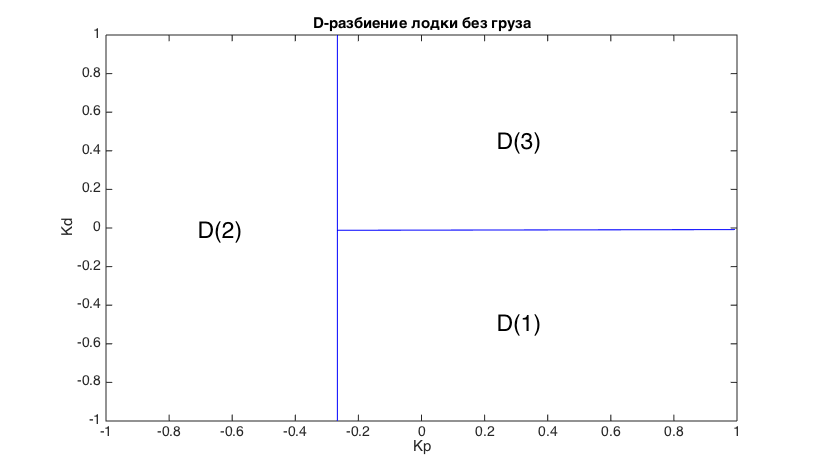
\includegraphics[width=1\linewidth]{images/d_part_no_cargo.png}}
	\caption{Области D-разбиения для лодки без груза}
\end{figure}

\begin{figure}
	\center{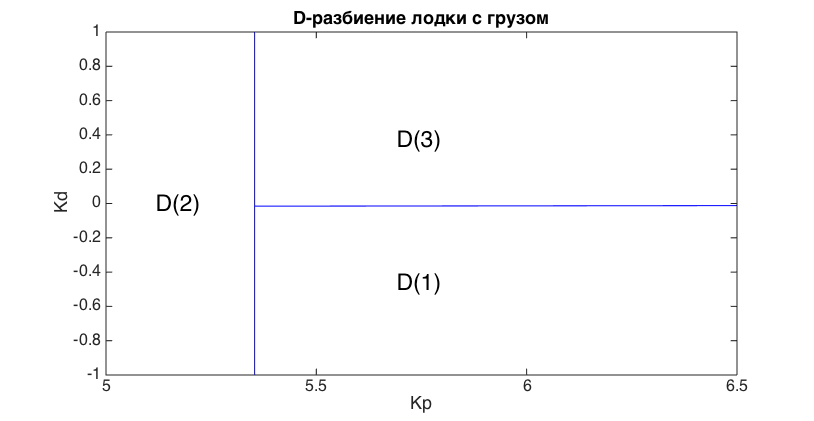
\includegraphics[width=1\linewidth]{images/d_part_cargo.png}}
	\caption{Области D-разбиения для лодки с грузом}
\end{figure}

Выбирая коэффициенты регулятора из области с тремя корнями в левой полуплоскости, мы будем получать устойчивые замкнутые системы. Дело за малым: выбрать какую-то осмысленную пару коэффициентов. В этой работе нас удовлетворит такая пара, при которой запас устойчивости по амплитуде будет больше 12 децибел, а запас устойчивойсти по фазе - больше 60 градусов. Вот пример таких коэффициентов для лодки с грузом (рис.~$\ref{fig:bode_stable_cargo}$). 

\begin{figure}
	\center{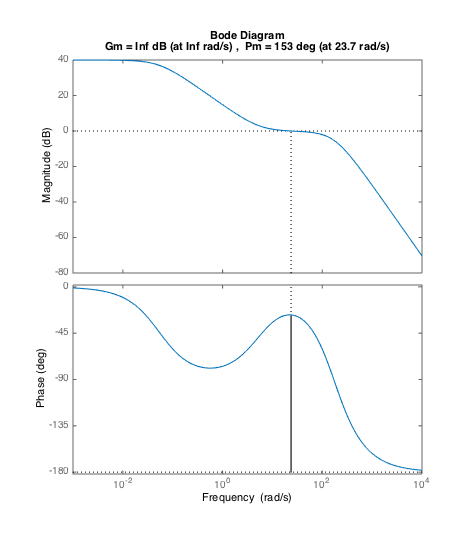
\includegraphics[width=1\linewidth]{images/bode_stable_cargo.png}}
	\caption{Запасы устойчивости лодки с грузом при $k_p=5.5$, $k_d=1$}
	\label{fig:bode_stable_cargo}
\end{figure}

\section{Результаты}

Была построена модель плавательной доски. Также был разработан алгоритм идентификации параметров модели. Подобран регулятор, стабилизирующий неустойчивую систему.


\section{Дальнейшие планы}

В дальнейшем хотелось бы автоматизировать процесс идентификации. Если это получится, то и алгоритм управления сразу же превратится в адаптивный.

\newpage

\bibliography{biblio/stable_bib}


\end{document}